\documentclass[lettersize,journal]{IEEEtran}
\usepackage{amsmath,amsfonts}
\usepackage{algorithmic}
\usepackage{algorithm}
\usepackage{array}
\usepackage[caption=false,font=normalsize,labelfont=sf,textfont=sf]{subfig}
\usepackage{textcomp}
\usepackage{stfloats}
\usepackage{url}
\usepackage{verbatim}
\usepackage{graphicx}
\usepackage{hyperref}
\usepackage{cite}
\usepackage{makecell}
\usepackage{epsfig}
\usepackage{epstopdf} 
\usepackage{gensymb}
\usepackage{multirow}
\usepackage{booktabs}
\usepackage{amssymb}
\usepackage{tabularx}
\usepackage{amsmath}
\usepackage{amssymb}
\usepackage{diagbox}
\usepackage[utf8]{inputenc}

% \makeatletter
\newcommand{\removelatexerror}{\let\@latex@error\@gobble}

\hyphenation{op-tical net-works semi-conduc-tor IEEE-Xplore}
% updated with editorial comments 8/9/2021

\begin{document}
\title{Active Object Detection for UAV Remote Sensing via Behavior Cloning and Enhanced Q-Network with Shallow Features}

\author{Zhuocheng Zou, Xikun Hu, and Ping Zhong, ~\IEEEmembership{Senior Member,~IEEE}
\thanks{Manuscript received xxx; This work was funded by National Natural Science Foundation of China(No.62301574) and the Science and Technology Innovation Program of HunanProvince(No.2024RC3119). (Corresponding author: Xikun Hu, Ping Zhong)



The authors are with the National Key Laboratory of Automatic Target Recognition, College of Electronic Science and Technology, National University of Defense Technology, Changsha 410073, China (e-mail: zzc@nudt.edu.cn; xikun@nudt.edu.cn; zhongping@nudt.edu.cn).}}

% The paper headers
% \markboth{Journal of \LaTeX\ Class Files,~Vol.~14, No.~8, August~2021}%

% \IEEEpubid{0000--0000/00\$00.00~\copyright~2021 IEEE}
% Remember, if you use this you must call \IEEEpubidadjcol in the second
% column for its text to clear the IEEEpubid mark.

\maketitle
\begin{abstract}
Object detection in Unmanned Aerial Vehicle (UAV) remote sensing imagery faces two critical challenges: the inability to effectively handle multi-scale targets and the difficulty in addressing partial occlusions, which significantly impact detection accuracy in real-world applications. To overcome these limitations, we propose an active object detection (AOD) method that dynamically adjusts viewing angles and scales during the detection process. Our key innovation lies in a novel architecture that uniquely combines shallow Feature Pyramid Network features with detector output bounding boxes, combining with a self-supervised learning framework. The technical originality of our approach is further enhanced by our two-stage learning methodology, which initially employs behavior cloning to establish robust foundational performance, followed by Q-learning fine-tuning to optimize detection strategies. To facilitate comprehensive evaluation, we introduce CARLA-AOD, a new benchmark dataset that encompasses 18 diverse scenarios across hemispheric space above targets, specifically designed for UAV remote sensing AOD applications. Extensive experimental validation demonstrates the effectiveness of our approach, achieving substantial improvements over baseline detectors across multiple datasets: 12.7\% on Small Airport, 14.0\% on Virtual Park, and 5.4\% on our CARLA-AOD dataset. The two-stage learning process proves particularly effective, with Q-learning fine-tuning providing an additional performance boost of up to 2.1\% beyond the behavior cloning baseline. Moreover, our method achieves a 60.2\% reduction in inference time compared to the state-of-the-art DCCL algorithm, making it particularly suitable for time-critical applications such as emergency response and real-time surveillance. The dataset is available at IEEE Dataport. \href{https://dx.doi.org/10.21227/t9r0-s152}{IEEE Dataport}.
\end{abstract}

\begin{IEEEkeywords}
Active Object Detection, UAV Remote Sensing, Reinforcement Learning, Behavior Cloning, Self-Supervised Learning.
\end{IEEEkeywords}

\section{Introduction}
\IEEEPARstart{O}{bject} detection, a fundamental task in computer vision, has gained significant prominence due to its wide-ranging applications. This task, which involves identifying and localizing specific objects within images or video streams, has become particularly valuable in the realm of remote sensing with the advent of Unmanned Aerial Vehicles (UAV). UAV-based remote sensing imagery offers unique advantages such as high spatial resolution, flexible data acquisition, and efficient coverage of large areas. Consequently, applying object detection to drone-captured imagery has opened up new possibilities in various domains, including urban planning \cite{remote2020}, agricultural monitoring \cite{estimating2014}, disaster response \cite{scheduling2021}, and environmental conservation\cite{reliability2019}.

Despite these advancements, existing UAV remote sensing image object detection methods predominantly adopt a passive processing mode. This approach involves passively receiving input images and applying pre-trained models for object detection without considering the dynamic nature of UAV flight or the specific characteristics of the scenario being observed. As a result, these methods often struggle to cope with challenges inherent to UAV-based imagery. For instance, the varying altitudes and angles at which UAVs capture images can lead to multi-scale targets \cite{empirical2021}, where objects of interest appear at different sizes and resolutions across a series of images. Additionally, the dynamic movement of UAVs can result in partial occlusions, where objects are temporarily obscured by the changing perspective of the UAV. These challenges, combined with other factors such as complex backgrounds typical in aerial imagery, significantly affect the performance and reliability of traditional object detection methods. The limitations of this passive approach become particularly evident in scenarios requiring real-time or near-real-time object detection, where the ability to quickly adapt to changing conditions is crucial.

To address these limitations, active object detection (AOD) \cite{hypothesis2013} has emerged as a promising solution. AOD refers to the process where the subject (e.g., UAV, robot) actively adjusts its perception strategy during the perception process to improve efficiency and accuracy. This dynamic approach represents a paradigm shift from traditional passive methods, enabling a more adaptive and intelligent form of object detection.

In the context of UAV-based remote sensing, AOD allows the system to optimize its view of areas of interest, effectively altering the scale of potential targets and changing its perception position relative to the targets , thereby increasing the likelihood of accurate detection.
By implementing these strategies, AOD significantly enhances the capabilities of UAV-based object detection systems. It allows for more robust performance in the face of challenges like multi-scale targets and partial occlusions. The ability to flexibly adjust flight paths and select optimal perception angles and positions leads to improved detection accuracy across a wide range of scenarios, which is particularly valuable in dynamic environments.

In recent years, AOD research has evolved along two primary trajectories: indoor robotics applications \cite{dataset2017, active2019, behavior2023, novel2021, active2022} and simple background scenarios \cite{enhancing2021,selfsupervised2022}. In indoor robotics, methods always rely heavily on horizontal camera movements for path planning, which limits their applicability to aerial scenarios where vertical perspective changes are crucial. Similarly, approaches designed for simple background scenarios make assumptions about object scale and background complexity that break down in aerial contexts.

The unique challenges of AOD in UAV remote sensing - including dramatic scale variations, complex backgrounds, and the need for rapid viewpoint adjustment - remain inadequately addressed. While Xu et al.'s Dynamic camera configuration learning (DCCL) \cite{dynamic2021} represented an initial attempt to tackle these challenges through reinforcement learning with detector neck features, their approach suffers from two key limitations: suboptimal performance due to the sole reliance on reinforcement learning, and computational inefficiency that prevents real-time deployment.

These limitations in existing work reveal three critical research gaps:
\begin{enumerate}
\item{The need for more efficient feature extraction that can handle the unique spatial characteristics of aerial imagery.}
\item{The lack of a learning framework that can effectively balance stability and exploration in complex aerial environments.}
\item{The absence of comprehensive evaluation benchmarks for UAV-specific AOD scenarios.}
\end{enumerate}

Building upon previous work, our work directly addresses these gaps and utilizes two key technologies: the Feature Pyramid Network (FPN), which is a feature extraction architecture that combines low-level detailed features with high-level semantic features, and behavior cloning, a technique that allows the model to learn from expert demonstrations by mimicking their decision-making process. 

Our key contributions are:
\begin{enumerate}
\item{A novel integration approach that uniquely combines the shallowest FPN features with detector output bounding boxes, introducing a self-supervised learning mechanism specifically designed for UAV-based AOD. This innovative architecture significantly improves the model's ability to capture fine-grained spatial details while maintaining computational efficiency, addressing a critical gap in existing UAV object detection systems.}
\item{An innovative dual-phase learning framework that introduces a new paradigm for AOD in complex UAV environments. Unlike existing methods that use either behavior cloning \cite{behavior2023} or reinforcement learning \cite{dataset2017, active2019,novel2021, active2022,enhancing2021,selfsupervised2022,dynamic2021} in isolation, our approach uniquely combines expert policy generation with behavior cloning in the initial phase, followed by a specialized Q-learning optimization phase. This novel integration enables robust performance in challenging UAV scenarios while minimizing the risks associated with random exploration.}
\item{The first comprehensive UAV-oriented benchmark dataset created using the CARLA simulator \cite{carla2017} that specifically addresses the unique challenges of aerial object detection. This dataset uniquely covers 18 diverse scenarios with complete hemispheric coverage above targets, providing a much-needed standardized evaluation platform for UAV-based AOD research.}
\end{enumerate}




\section{Related Work}

\subsection{Active Object Detection}
AOD dynamically adjusts perception strategies during the perception process, enhancing efficiency and accuracy compared to traditional passive methods, making it a promising solution for overcoming inherent limitations in object detection. AOD methods can be divided into two categories: single-object AOD and multi-object AOD.

Single-object AOD methods typically utilize observation images and detection boxes for decision-making. Han et al. \cite{active2019} proposed a Dueling DQN structure with divided advantage functions for action type and range, though this approach introduced training instability. Liu et al. \cite{active2022} selected optimal actions based on the distance between image center and detection box center, as well as target box area, calculating rewards using a greedy method, but this approach proved unsuitable for UAV remote sensing scenarios requiring multiple object detection. Liu et al. \cite{behavior2023} conducted imitation learning based on expert data obtained through shortest path search, requiring single object positioning to determine end states for optimal path generation. Jiang et al. \cite {Azimuth2024} performed active target recognition by combining UAV SAR images with historical image sequences, but only adjusted observation azimuth angle, limiting application scenarios.

While single-object AOD methods have their specific application scenarios, they struggle to meet the demands of multi-target detection in UAV remote sensing contexts. Recognizing these limitations, as single-object detection methods gradually matured, researchers began exploring multi-object AOD, introducing new challenges in perception and action selection. Fang et al. \cite{enhancing2021,selfsupervised2022} improved upon \cite{active2019} to apply it to multiple regular objects. In \cite{enhancing2021}, they adopted a two-stage training approach to progressively predict action type and range, alleviating the training instability issues in \cite{active2019}. In \cite{selfsupervised2022}, they pre-trained the feature extraction network using InfoNCE loss to further enhance generalization performance. However, these studies were conducted in relatively simple backgrounds with fixed observation scales, making adaptation to complex UAV remote sensing scenarios challenging. Xu et al. \cite{dynamic2021} directly utilized intermediate features from the detector's feature extraction network combined with historical actions for decision-making, assigning rewards based on detection score differences between consecutive frames and total steps taken. However, using all detector-provided features led to efficiency deficiencies, which is problematic in UAV AOD scenarios where efficiency is crucial. Overall, there remain gaps in current multi-object AOD approaches for UAV remote sensing applications, particularly regarding efficiency.

\begin{figure}[!t]
    \centering
    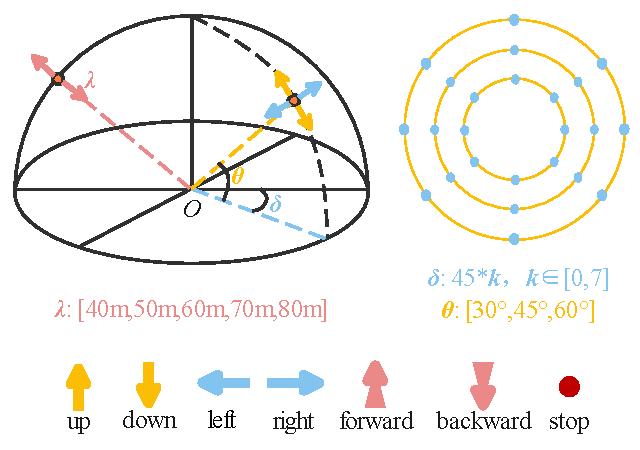
\includegraphics[width=0.45\textwidth]{fig/state_action.pdf}
    \caption{State and Action Space of AOD. The state of the camera can be denoted by longitude $\delta$, latitude $\theta$, and scale $\lambda$, which can be controlled by 7 types of actions: up, down, left, right, forward, backward and stop.}
    \label{Stat_Action}
\end{figure}

\subsection{Active Object Detection Datasets}
Based on different sources, AOD datasets can be divided into natural scenario AOD datasets and remote sensing scenario AOD datasets.

Currently, the publicly available natural scenario datasets used for AOD include: the AVD (Active Vision Dataset) indoor active vision dataset constructed by Ammirato et al.\cite{dataset2017} and the Gibson dataset built by Xia et al.\cite{gibson2018}. Among them, the AVD dataset is currently the most widely used AOD dataset. The dataset consists of 9 room environments, where each room is divided into multiple rectangular spaces with center points 30 cm apart, simulating discrete positions where robots might exist in the room. At each spatial point, 12 images are captured at 30\degree directional angle intervals, including both visible light images and depth images, thus forming the dataset.

Regarding remote sensing AOD datasets, there are two representative datasets: Small Airport (SA) and Virtual Park (VP)\cite{dynamic2021}, both of which are simulated images. As shown in Fig. \ref{Stat_Action}, these two datasets consider longitude, latitude, and distance, with the sensor viewpoint always pointing towards the center point, and the sensor position only covering 1/4 of the hemisphere space. The VP dataset also considers the impact of different lighting conditions on object detection accuracy.

Currently, AOD datasets for UAV remote sensing data remain scarce with existing datasets limited to single-scenario environments (airport and park scenarios), lacking scenario diversity. They also contain a limited number of object instances, which restricts model robustness. Moreover, both datasets only cover the upper quarter hemisphere, providing incomplete environmental perception and limiting their practical applications in real-world deployment scenarios.










\section{Methodology}
Implementing AOD in complex environments requires a system capable of dynamically adjusting viewpoints and optimizing detection performance. Our approach achieves efficient object detection by integrating feature extraction, camera control strategies, and self-supervised learning mechanisms. To help readers better understand our method, we first summarize the overall workflow of the model through a high-level diagram in Fig. \ref{Overview} before delving into the problem formulation and the technical details of each module.

In the following sections, we will formulate the problem of AOD in UAV remote sensing and elaborate on three key aspects: the network architecture, the behavior cloning based on the A-star search algorithm, and the implementation of the policy network.

\begin{figure}[!t]
    \centering
    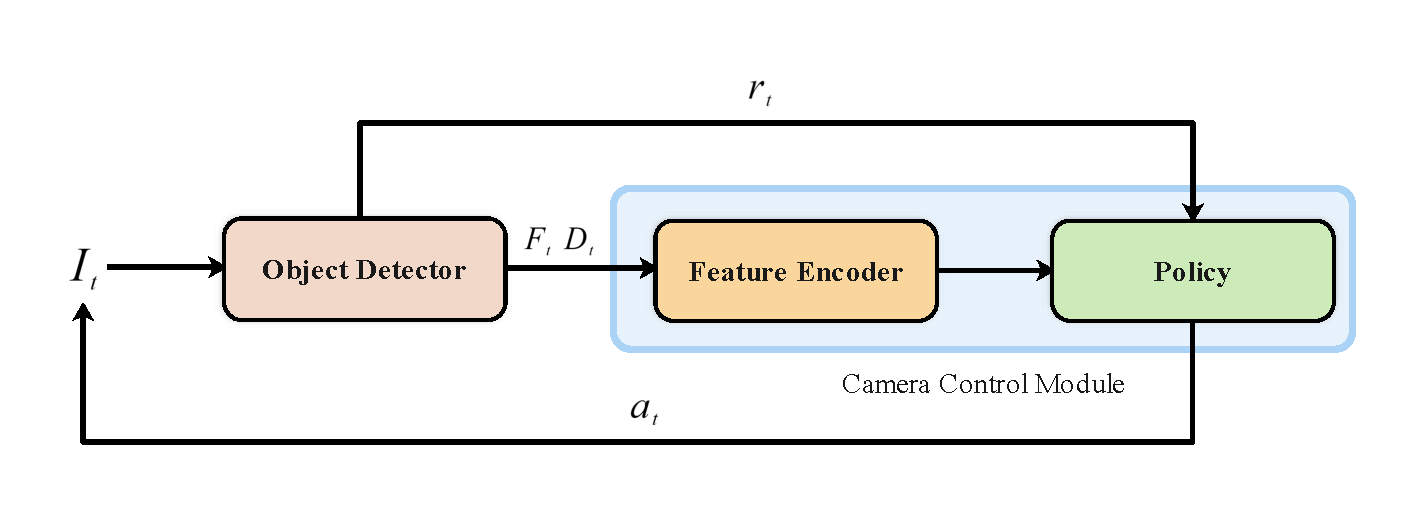
\includegraphics[width=0.45\textwidth]{fig/overview.pdf}
    \caption{The Overview of the Proposed Framework}
    \label{Overview}
\end{figure}

\begin{figure*}[!ht]
	\centering
	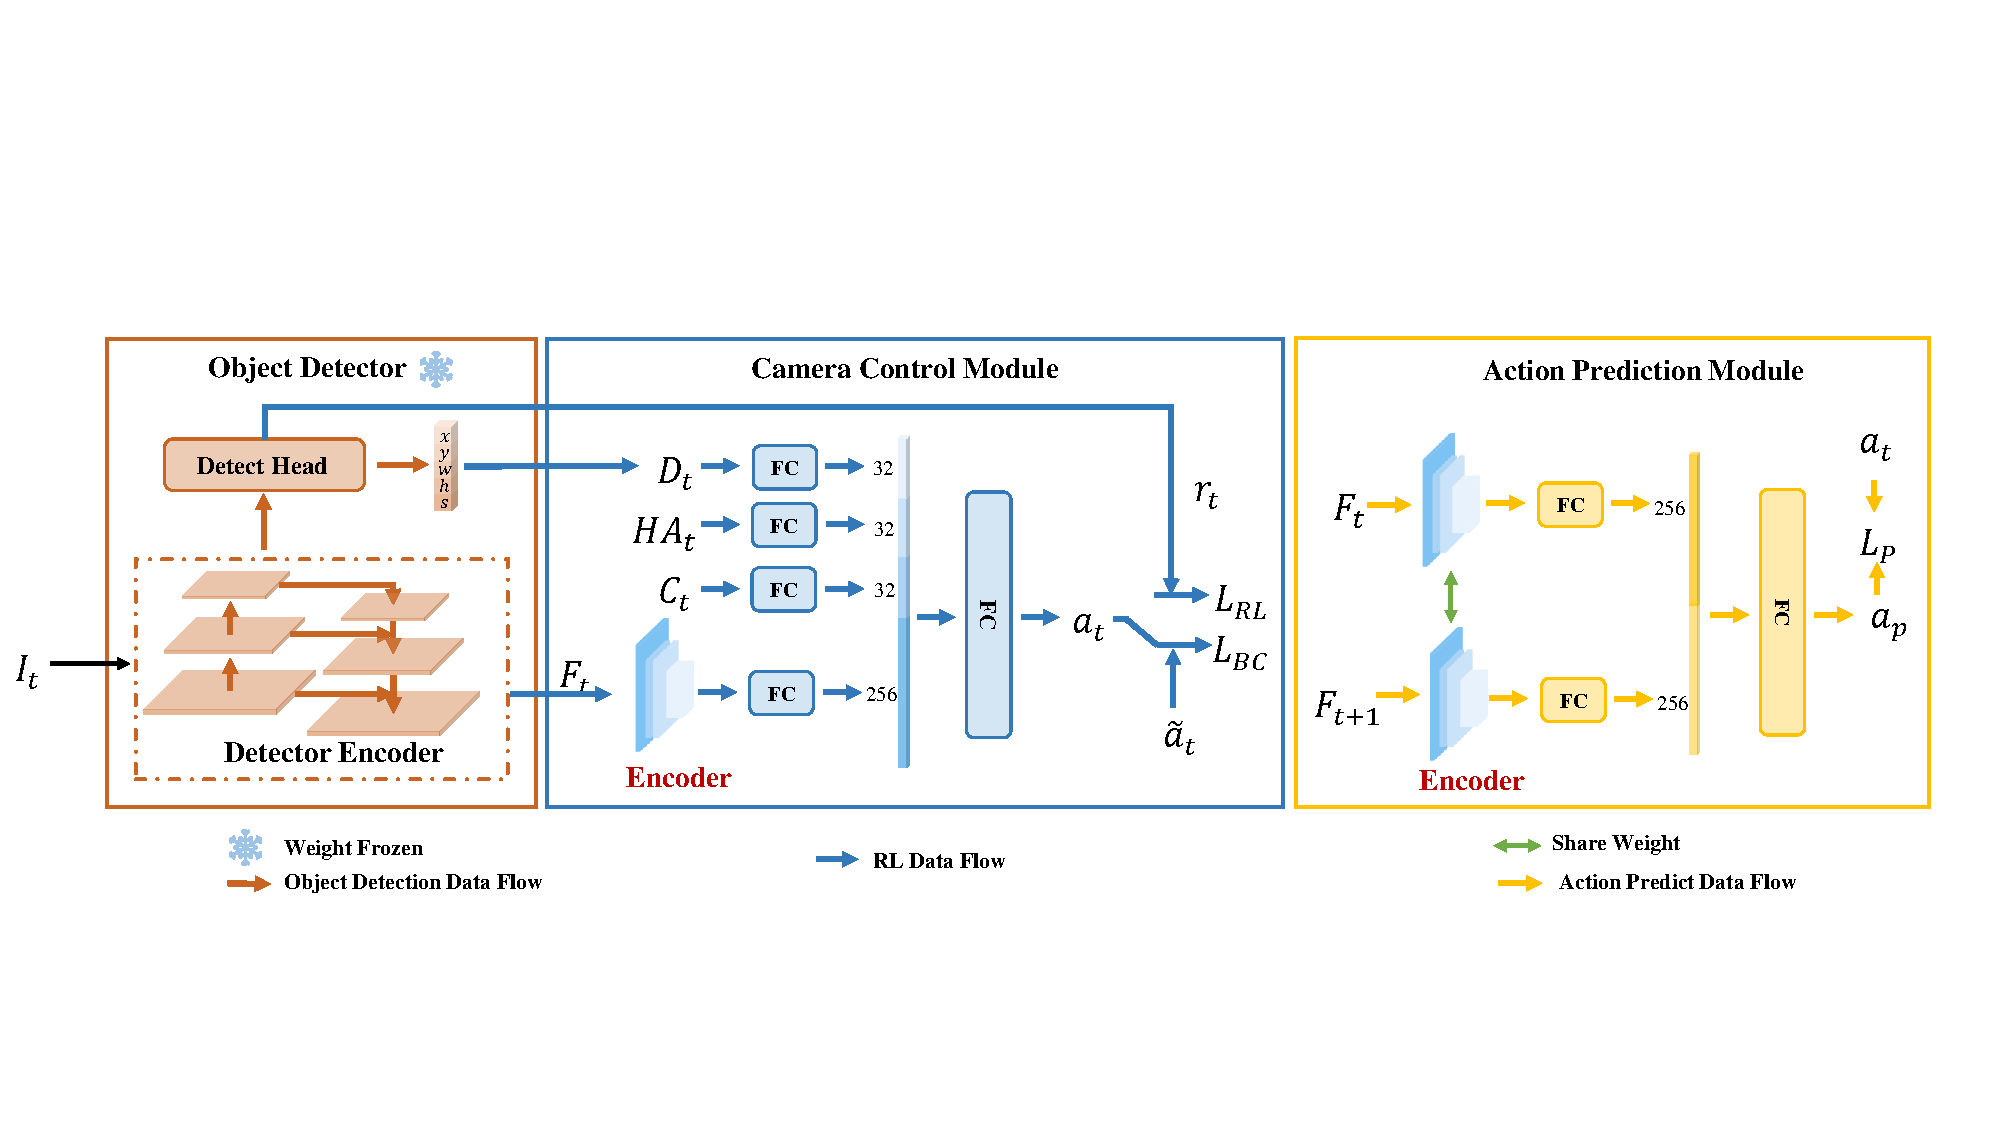
\includegraphics[clip=true, width=1.0\textwidth]{fig/overview2.pdf}
	\caption{The architecture of the proposed framework consists of three data flows: object detection flow, reinforcement learning (RL) flow, and action prediction flow..  In the object detection flow, the image at time $t$ is processed to obtain shallow features $F_t$ and detection results $D_t$, with pre-trained and frozen detector weights.  In the RL flow, detection results $D_t$, historical actions ${HA}_t$, position encoding $C_t$, and feature encoded from $F_t$ through the encoder are independently processed through FC layers to output action $a_t$.  The RL data flow undergoes training in two stages: in stage one, supervised training is performed using expert actions $\tilde{a}_t$ obtained from A-star and combining them with behavior cloning techniques;  and in stage two, reinforcement learning is used for fine-tuning, utilizing the detector to generate reward $r_t$ for training.  In the action prediction flow, current features $F_t$ and next-step features $F_{t+1}$ are encoded and concatenated to predict action $a_p$, which serves as an estimation of the actual action $a_t$.}
	\label{Architecture}
\end{figure*}

\subsection{Overview}
The framework of our proposed model is illustrated in Fig. \ref{Overview}, which provides a high-level overview of the entire system. Our novel approach integrates an object detector with a camera control module to dynamically adjust the UAV's viewpoint and optimize detection performance. Specifically, the pre-trained object detector processes the current image to extract relevant features $F_t$ and detected object results $D_t$, which are then fed into the camera control module. These outputs are not only used to determine the optimal adjustment action $a_t$ but also to generate the reward signal $r_t$ that evaluates the detection performance at each step. Finally, the camera control module is trained through a two-stage process: initial behavior cloning followed by reinforcement learning fine-tuning. The overall workflow is designed to enhance detection accuracy by actively optimizing the UAV's viewpoint, making our method particularly effective in challenging remote sensing scenarios.

\subsection{Problem Formulation}
AOD in remote sensing represents a paradigm shift from traditional approaches, aiming to dynamically optimize the process of object detection in complex aerial environments. This method leverages a decision-making model that continuously adjusts the UAV camera states, specifically its view and scale, based on the current image input until the optimal state for object detection is achieved, thereby enhancing both the effectiveness and adaptability of detection in varied and challenging scenarios.

The dynamic and sequential nature of AOD aligns well with the framework of a Markov Decision Process (MDP), which is commonly handled by reinforcement learning methods. This mathematical model for decision making consists of six fundamental components: a state space $S$, an action space $A$, a reward function $R$, transition probabilities $P$, a discount factor $\gamma$, and a policy $\pi$. 

These components collectively describe the environment, possible actions, feedback mechanism, state transitions, long-term reward considerations, and decision strategy respectively. The process unfolds as follows:
\begin{enumerate}
\item{State: At each time step $t$, the agent (UAV) observes the current state $s_t$.}
\item{Action Generation: According to policy $\pi$, the agent generates an action $a_t = \pi(s_t)$.}
\item{State Transition: This action causes a transition to a new state $s_{t+1} = P(s_t, a_t)$.}
\item{Reward: The agent receives a reward $r_t = R(s_t, a_t)$ from the environment.}
\end{enumerate}

The core objective of the reinforcement learning algorithm in AOD is to learn an optimal camera control strategy that maximizes the cumulative discounted rewards, expressed as $U_t = \sum_{i=t}^{\infty}{\left( \gamma ^{i-t}r_i \right)}$, where $\gamma \in [0,1]$ is the discount factor that determines the present value of future rewards.

As depicted in Fig. \ref{Stat_Action}, inspired by the work of \cite{dynamic2021}, we have discretized the state space $S$. Range of motion of the camera is constrained within a hemispherical space positioned above the target area $O$, with the camera consistently oriented towards $O$. We can adjust the camera state across three key dimensions: longitude, latitude, and scale. The longitude $\delta$ is defined as $\delta = 45\degree * k$, where $k \in [0,7]$, allowing for a full 360\degree horizontal rotation in 45\degree increments. The latitude $\theta$ takes values in the set $\left\{30\degree, 45\degree, 60\degree \right\}$, representing different vertical angles of view. The scale $\lambda$ corresponds to the distance from the target, with values in the set $\left\{40m, 50m, 60m, 70m, 80m \right\}$, allowing for varying levels of detail and field of view.

Additionally, our action space $A$ comprises seven distinct control actions: up, down, left, right, forward, backward, and stop. These actions allow the UAV to change state in the discretized hemispherical space effectively, adjusting its position and scale to optimize object detection performance. This formulation provides a comprehensive framework for modeling and solving the AOD problem in UAV-based remote sensing.

\begin{figure}[!t]
    \centering
    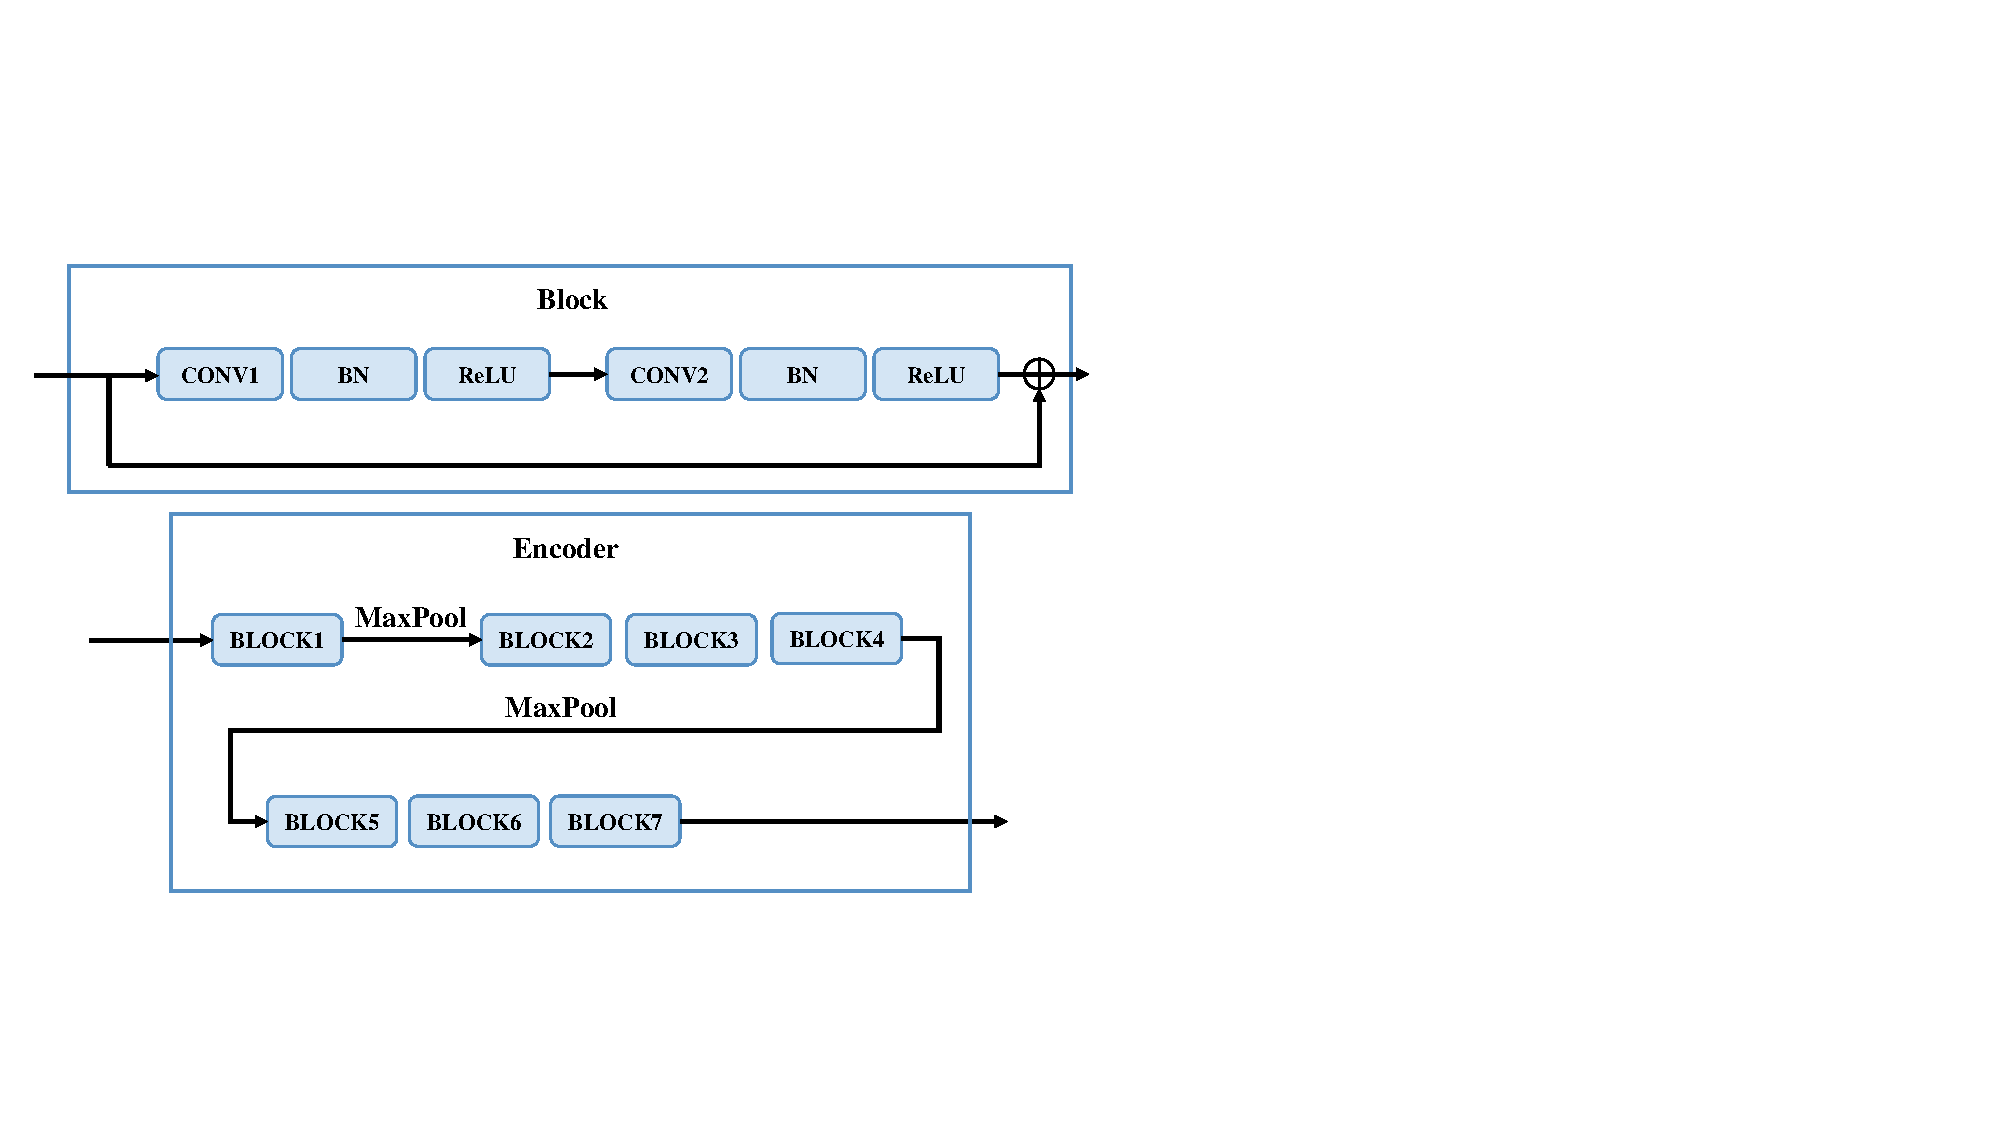
\includegraphics[width=0.45\textwidth]{fig/encoder.pdf}
    \caption{The Architecture of the Encoder}
    \label{Encoder}
\end{figure}

\subsection{Network Architecture}

Our approach builds upon and significantly improves the DCCL framework through several key architectural innovations. While DCCL utilizes all feature layers from the detector's neck for decision-making, our method strategically focuses on the shallowest FPN features, which we found to be most relevant for AOD tasks. This targeted feature selection offers two main advantages over DCCL: improved computational efficiency by reducing the feature processing overhead, and enhanced spatial precision by leveraging the rich positional and boundary information preserved in shallow features.  Furthermore, where DCCL relies solely on feature-based decision making, our architecture introduces a novel integration of our self-supervised action prediction module with shallow features, which enables more robust and context-aware decision making compared to DCCL's feature-only approach.

As shown in Fig. \ref{Architecture}, at time $t$, the camera control module processes a multi-dimensional state value $S_t$, which is comprised of four key components: $F_t$, the shallowest layer FPN features extracted from the input image $I_t$ by the object detector; $D_t$, the detected object bounding box coordinates with corresponding confidence scores; $C_t$, the camera state; and ${HA}_t$, the historical actions.
The structure of the encoder, shown in Fig. \ref{Encoder}, consists of 7 sequentially connected Blocks, including two MaxPool operations. Each Block comprises two convolutional layers, two batch normalization layers, and two ReLU activation layers, as well as a residual connection. $F_t$ undergoes processing through the encoder, yielding a 256-dimensional vector.
Concurrently, the other three inputs ($D_t$, $C_t$, and ${HA}_t$) are transformed into 32-dimensional vectors via fully connected layers. These vectors are then concatenated and fed into a final fully connected layer which transforms the 352-dimensional input through two fully connected layers (352→128→7) with ReLU activations. The output 7-dimensional vector represents the probability distribution over possible actions, from which we select the action with the highest probability value as the optimal action $a_t$.

Each component of $S_t$ plays a crucial role in our network architecture. For the feature $F_t$ extracted by encoder of detector, our approach diverges from DCCL in that we exclusively use the shallowest layer features from neck of the detector, rather than all output features.
To provide a more comprehensive understanding of this decision, we conducted a detailed analysis of the feature maps extracted from different levels of the FPN. As shown in Fig. \ref{FPN_features}, we visualize the feature maps from the shallowest layer to the deepest layer extracted from the object detector.


The shallow-level feature map (Fig. \ref{FPN_features} b) retains a high spatial resolution compared to the input image. This layer is rich in detailed information, preserving clear object boundaries and contours, which is highly beneficial for accurate localization and identification of targets. The shallow features also capture strong local texture and edge information, enabling the model to effectively extract fine-grained visual cues.
The mid-level feature maps (Fig. \ref{FPN_features} c, d) have a lower spatial resolution, but they strike a balance between local and global features. While the object boundary information becomes more blurred, these mid-level features are able to encode richer semantic information about the overall scene.

The deep-level feature maps (Fig. \ref{FPN_features} e, f) have an even lower spatial resolution. The object boundary and contour details become severely degraded, but the global semantic information is more prominent. These deep features are more suitable for high-level semantic understanding tasks, such as scene classification and object recognition.
This decision to use the shallowest layer features is based on the observation that these shallow features contain most of the positional relationships and object contour information crucial for AOD, potentially accelerating the execution speed of the model by reducing the volume of data to be processed.

The detected object information $D_t$ is derived from several horizontal bounding boxes extracted from each image. Each box is encoded as a 5-tuple (x, y, w, h, s), where (x, y) represents the center position of the box, (w, h) denotes its width and height, and s indicates the confidence score. These tuples are concatenated to form a 100-dimensional vector $D_t$, zero-padded if necessary, providing a comprehensive representation of both the spatial layout and detection confidence of objects in the scenario. The camera state $C_t$ encapsulates the current camera information (24 views, 5 scales), offering comprehensive information about the current perspective and zoom level of the observed scenario. The historical actions ${HA}_t$ are constructed by concatenating the one-hot encodings of the three most recent actions, allowing the model to understand the recent decision sequence and potentially make more coherent action choices.

\begin{figure}[!t]
    \centering
    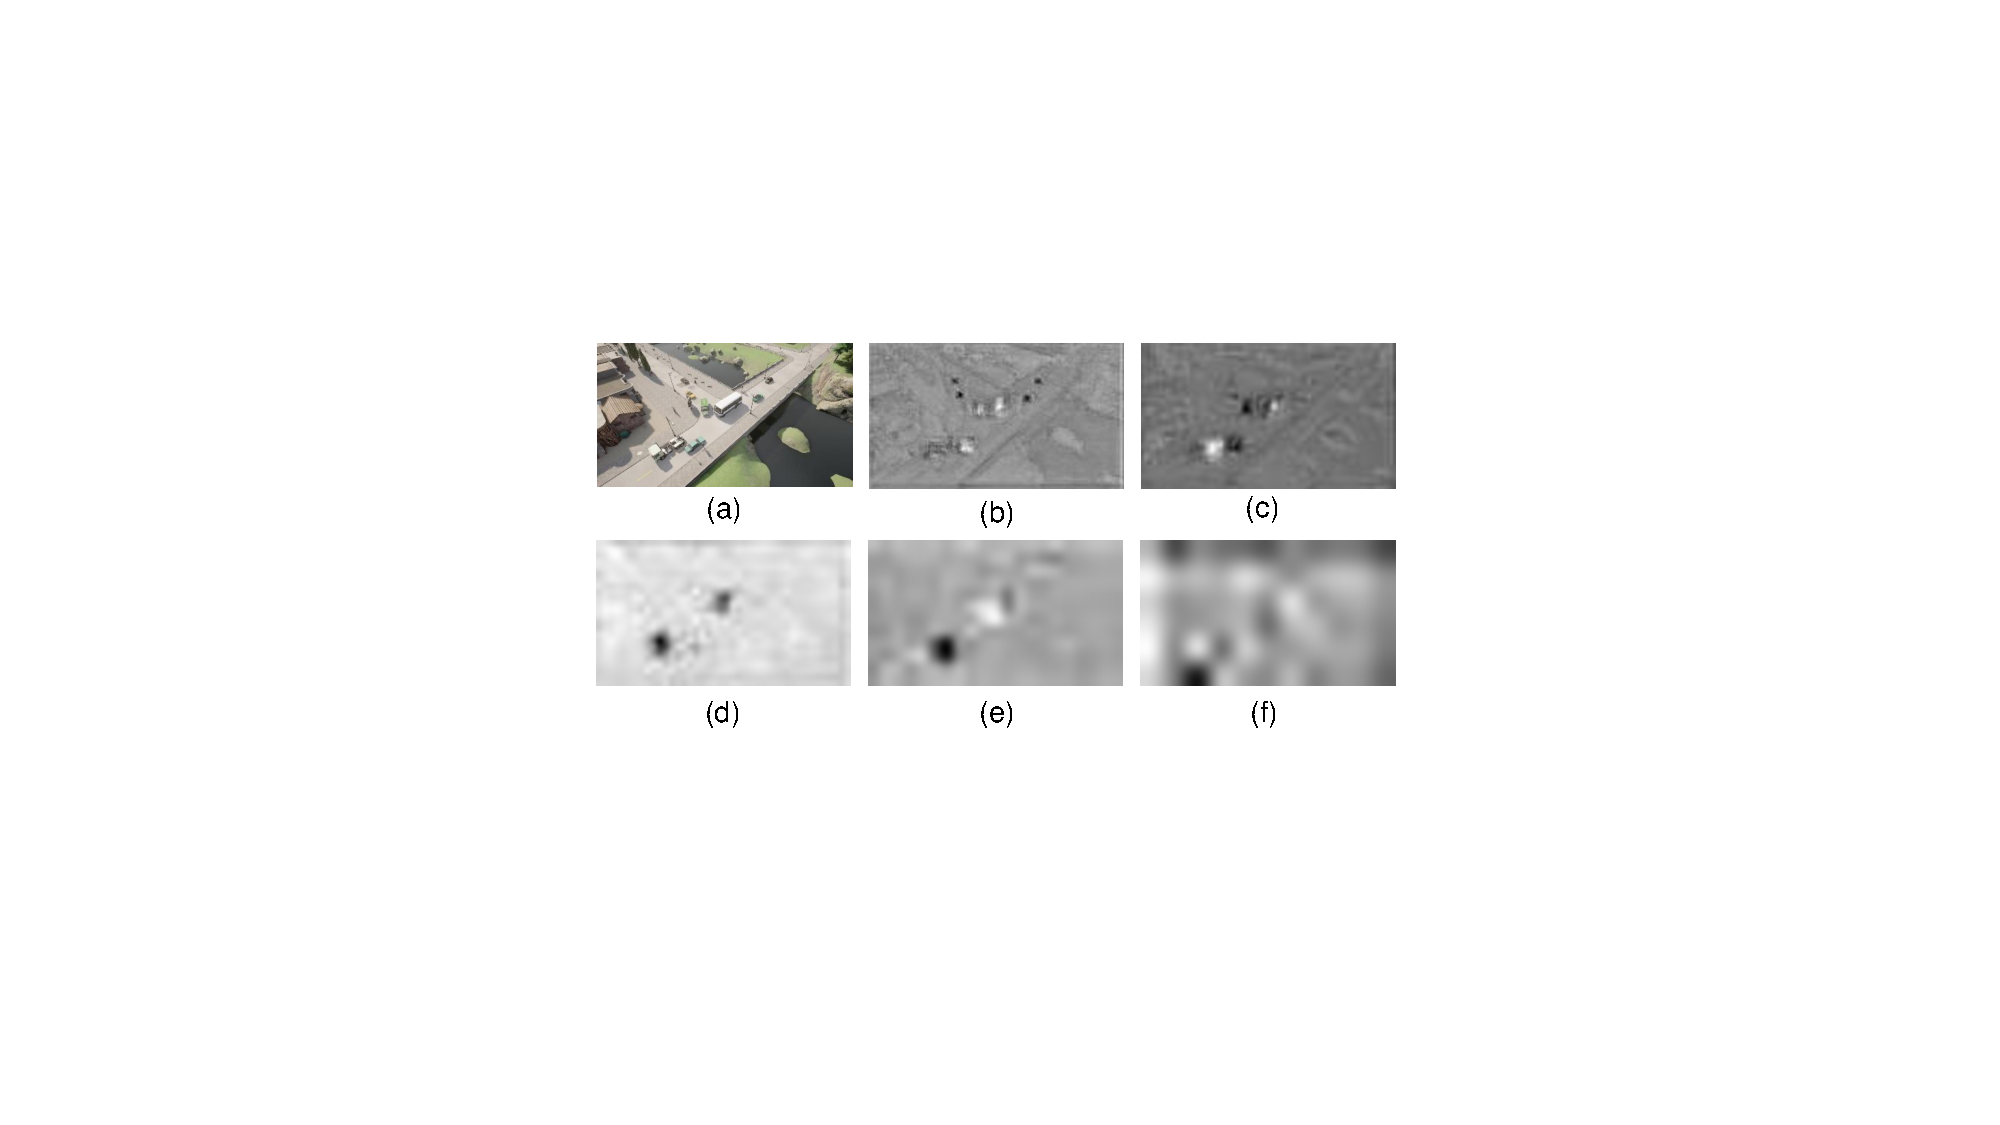
\includegraphics[width=0.45\textwidth]{fig/shallow_feature.pdf}
    \caption{Visualization of FPN Feature Maps. (a) Original Image. (b-f) Shallowest FPN Feature Map to Deepest FPN Feature Map.}
    \label{FPN_features}
\end{figure}

To further enhance the  feature extraction capabilities of encoder for AOD, we incorporate a self-supervised auxiliary task into our network architecture. This task is implemented through an action prediction module, as illustrated in Fig. \ref{Architecture}. This task processes the current image $I_t$ through the model to output action $a_t$, leading to the subsequent image $I_{t+1}$. The feature vectors of these two images are concatenated and passed through two fully connected layers (512→128→7) with ReLU activations to obtain the probability distribution $a_p$ of the action, serving as a prediction for $a_t$. The prediction loss $L_{P}$ is calculated using cross-entropy between the predicted and expert actions, as shown in Eq. \ref{pred_loss}:
\begin{equation}
L_{P}\left( a_t,a_p \right) =-\sum_{i=1}^n{a_{t}^{i}*\log \left( a_{p}^{i} \right)}
\label{pred_loss}
\end{equation}

By learning to predict actions between consecutive frames, this approach implicitly introduces an attention mechanism, enabling the model to focus on dynamic features related to scenario changes. This enhancement in understanding scenario dynamics is expected to improve the ability of the model to make intelligent and coherent decisions in AOD tasks, potentially increasing both detection accuracy and efficiency. It is noteworthy that the action prediction module is only active during the training phase and is not utilized during inference, thereby ensuring efficient model operation in practical applications. 

The overall architecture of the model can be viewed as an end-to-end system that integrates feature extraction, object detection, state encoding, decision-making, and self-supervised learning, allowing for comprehensive consideration of visual features, detection results, camera configuration, and historical actions in the decision-making process.

\subsection{Behavior Cloning Based on A-star}
In Fig. \ref{Architecture}, given the challenges posed by complex backgrounds, behavior cloning plays a crucial role in guiding effective learning in the Camera Control Module. Behavior cloning provides a structured solution by leveraging expert demonstrations to supervise initial training, which accelerates the learning process and reduces the trial-and-error phase typically associated with reinforcement learning.

We adopted this approach after careful consideration of alternative imitation learning techniques. Unlike Generative Adversarial Imitation Learning (GAIL) \cite{generative2016}, which requires complex adversarial training between policy and discriminator networks, behavior cloning offers a more direct and stable approach through supervised learning, establishing a reliable foundation policy. Similarly, compared to Inverse Reinforcement Learning (IRL) \cite{algorithms2000} techniques that first infer reward functions from demonstrations and then optimize policies, behavior cloning's direct policy imitation provides faster convergence with fewer samples—a significant advantage in UAV remote sensing where expert demonstrations represent optimal viewing positions. While behavior cloning may lead to overfitting to expert actions, our two-stage learning approach addresses this concern by using reinforcement learning to fine-tune the policy, allowing the agent to dynamically optimize based on reward feedback, balancing initial rigidity with long-term flexibility.

To implement behavior cloning effectively, we employ the A-star algorithm to generate expert demonstrations, which serve as the foundation for this imitation learning process. The A-star algorithm plays a crucial role in improving detection accuracy by optimally guiding the UAV camera to viewpoints that maximize mean Average Precision (mAP) \cite{microsoft2014}.  This is achieved through a carefully designed heuristic approach that combines both local and global optimization.  For each scenario, we first construct a comprehensive mAP evaluation matrix $M(N_\delta,N_\theta,N_\lambda)$ that quantifies detection performance across all possible camera states, defined by longitude $\delta$, latitude $\theta$, and scale $\lambda$.  By identifying the three points with highest mAP values as endpoint targets, we establish optimal viewing positions that serve as navigation goals for the UAV.

The algorithm's effectiveness in improving mAP stems from its intelligent path-finding mechanism that uses a heuristic cost function $H(P)=M(E_0)-M(P)$, where $P$ represents the current position and $E_0$ is the nearest endpoint.  This heuristic guides the camera trajectory by balancing two critical factors: the immediate detection performance at the current position $M(P)$ and the potential gain in reaching the optimal endpoint $M(E_0)$.  This dual consideration ensures that the algorithm not only pursues paths leading to high-performance viewpoints but also maintains reasonable detection quality during the transition, resulting in better overall mAP scores. The complete implementation of this approach is detailed in Algorithm \ref{alg:alg1}.

Moreover, the A-star approach's ability to improve mAP is enhanced by its systematic exploration of the state space.  Rather than randomly searching for better viewpoints, it efficiently evaluates potential paths by considering both the cost of reaching the current position and the estimated cost to the goal.  This informed search strategy allows the algorithm to quickly identify and traverse paths that lead to viewpoints offering superior detection performance, while avoiding less promising regions of the search space.  The resulting camera trajectories effectively balance exploration of promising viewpoints with exploitation of known high-performance positions, leading to consistent improvements in overall detection accuracy as measured by mAP.

From paths computed by A-star, we derive corresponding actions for each step, resulting in optimal action labels $\tilde{a}_t$ for each time $t$. These labels, which represent the expert's decisions, serve as a gold standard for the agent. To facilitate behavior cloning, we constrain the model's output actions ${a}_t$ to align with these optimal labels through a cross-entropy loss $L_{BC}$, as detailed in Eq. \ref{bc_loss}. The total loss for behavior cloning is then expressed as the sum of $L_{BC}$ and $L_{P}$, as shown in Eq. \ref{loss1}.

This comprehensive approach to behavior cloning allows us to generate high-quality expert trajectories that guide the agent towards optimal viewing positions. By leveraging the efficiency of the A-star algorithm in path finding and the mAP-based heuristic for evaluating camera positions, we ensure that the agent learns from trajectories that maximize detection performance.

\begin{figure}[!t]
\begin{algorithm}[H]
\caption{A-star}\label{alg:alg1}
\begin{algorithmic}[1]
\STATE $\textbf{Input: }$Start point $S$ and End point $E_0$
\STATE $\textbf{Output: }$a minimum-cost path leading to $E_0$
\STATE $\textbf{Initialize:}$  minheap $\mathbf{pq}= [(0,S)] $ ,
actual path cost buffer $\mathbf{g}=\left\{ {S:0} \right\},
$ parent buffer of node $\mathbf{P}=\left\{ S:None \right\}$  
and close list $\mathbf{C}=\left[  \right]$
\STATE \textbf{while} $\mathbf{pq}$: % While loop starts
\STATE \hspace{0.5cm} $\_, Cur$=$\mathbf{pq}$.pop()
\STATE \hspace{0.5cm} $\mathbf{C}$.append($Cur$)
\STATE \hspace{0.5cm} \textbf{if} $Cur$==$E_0$: % If statement starts
\STATE \hspace{1.0cm} path=[]
\STATE \hspace{1.0cm} while $Cur$ is not None: % Inner while loop starts
\STATE \hspace{1.5cm} path.append($Cur$)
\STATE \hspace{1.5cm} $Cur=\mathbf{P}[Cur]$
\STATE \hspace{1.0cm} \textbf{end while} % Inner while loop ends
\STATE \hspace{1.0cm} \textbf{return} path.reverse() % Inner while loop ends
\STATE \hspace{0.5cm} \textbf{end if} % If statement ends
\STATE \hspace{0.5cm} \textbf{for} each $neighbor$ of $Cur$: % For loop starts
\STATE \hspace{1.0cm} \textbf{if} $neighbor$ is valid \textbf{and} not in $\mathbf{C}$ : % If statement starts
\STATE \hspace{1.5cm} $f=\mathbf{g}[Cur]+H(neighbor)$ 
\STATE \hspace{1.5cm} \textbf{if} $neighbor$ not in $\mathbf{g}$ \textbf{or }$f<\mathbf{g}[neighbor]$ : % Nested if starts
\STATE \hspace{2.0cm} $\mathbf{g}[neighbor]=f$
\STATE \hspace{2.0cm} $\mathbf{pq}$.push(($f,neighbor$))
\STATE \hspace{2.0cm} $\mathbf{P}[neighbor]=Cur$
\STATE \hspace{1.5cm} \textbf{end if} % Nested if ends
\STATE \hspace{1.0cm} \textbf{end if} % If statement ends
\STATE \hspace{0.5cm} \textbf{end for} % For loop ends
\STATE \textbf{end while} % While loop ends
\end{algorithmic}
\end{algorithm}

\end{figure}

\begin{equation}
L_{BC}\left(\tilde{a}_t,{{a}}_t\right)=-\sum_{i=1}^{n}{{\tilde{a}_t}^i\ast\log{\left({{a}}_t^i\right)}}
\label{bc_loss}
\end{equation}

\begin{equation}
L_{1}=L_{BC}+L_P
\label{loss1}
\end{equation}

\subsection{Implementation of Policy Network}
Building upon the foundation established through behavior cloning, we implement a policy network using the Double Deep Q-Network (DDQN) \cite{deep2016}. 
This value-based approach enables optimal action selection by evaluating the value of various actions in the current state.
The DDQN algorithm optimizes the policy network parameters by minimizing the reinforcement learning loss. This loss is defined as the temporal difference between the Q-value of the current time $Q_{\vartheta}(s_t, a_t)$ and the target Q-value $q_t^{tgt}$, where $Q_{\vartheta}(s_t, a_t)$ is computed by the policy network $\vartheta$ and $q_t^{tgt}$ is derived from the target network $\psi$ and reward function $R$. The target network is periodically updated to align with the policy network. The loss function is formulated as Eq. \ref{rl_loss}.
\begin{equation}
    \begin{aligned}
        L_{RL}\left( \vartheta ,\psi \right) &=\frac{1}{2}\lVert q_{t}^{tgt}-Q_{\vartheta}\left( s_t,a_t \right) \rVert _{2}^{2}\\
        q_{t}^{tgt}=R_t +&\gamma Q_{\psi}\left( s_{t+1},\underset{a}{argmax}Q_{\vartheta}\left( s_{t+1},a \right) \right)
    \end{aligned}
    \label{rl_loss}
\end{equation}

The reward function $R_t$, crucial for providing feedback on chosen actions, is defined as Eq. \ref{reward_function}.
\begin{equation}
    R_t=\begin{cases}
        sign\left( m_{t+1}-m_t \right) -\alpha O\left( a_t,a_{t-1} \right)&		t<T\\
        -3+5\mathbb{I}\left( m_t\geq \mu \right)&		t=T\\
    \end{cases}
    \label{reward_function}
\end{equation}
The function $sign(x)$ returns 1 when $x > 0$, and -1 otherwise, effectively rewarding improvements in detection performance, where $m_t$ represents the detector's performance evaluation (mAP) of the image at time $t$.
To discourage oscillatory behavior, $O(a_t,a_{t-1})$ penalizes the use of opposite actions, returning 1 when actions are opposite and 0 otherwise, with $\alpha$ serving as the penalty coefficient.
At the terminal step $T$, the reward incorporates an indicator function $\mathbb{I}(\cdot)$, which equals 1 when its argument is true and 0 otherwise.
This function compares the final performance $m_T$ with $\mu$, the mean value of $m_t$, providing an additional reward if the final performance exceeds the average.

In summary, for $t < T$, the reward depends on performance improvement and action coherence.
At $t = T$ (episode end), the final reward is based on whether the performance of the last selected image exceeds the average.
This reward strategy encourages the model to select better-performing images and avoid oscillatory behavior.

Similarly, the total loss for the reinforcement learning stage, denoted as \( L_2 \), is the sum of \( L_P \) and \( L_{RL} \):

\begin{equation}
L_2 = L_P + L_{RL}
\end{equation}






\section{Experiments}
In this section, we validate and evaluate the performance of our proposed framework on both AOD datasets SA, VP \cite{dynamic2021} and our newly proposed dataset. Our evaluation encompasses quantitative metrics, including mAP and running speed, as well as visualizations of results of our approach.

\subsection{Datasets}

We conduct experiments on three datasets: the SA, VP dataset and our proposed CARLA-AOD dataset. The SA dataset contains 12 aircraft categories and is composed of 4,500 remote sensing images, including 90 different scenarios. The camera in SA has 10 perspectives and 5 scales. The VP dataset contains 5 vehicle categories and is composed of 5,000 remote sensing images, including 20 different scenarios. While the original VP dataset includes 5 brightness levels, in our experiments we focus solely on perspective and scale variations, thus using only one brightness level. The camera in VP has 10 perspectives and 5 scales.

Our proposed AOD dataset, CARLA-AOD, illustrated in Fig. \ref{dataset}, is created by the CARLA autonomous driving simulator. It consists of 2,160 images taken from 18 diverse scenarios, including multiple urban and rural scenarios. CARLA-AOD contains 4 vehicle categories (Car, Truck, Van, Bus) and follows the framework described in Section 2, encompassing 24 views (composed of 3 latitudes and 8 longitudes) and 5 scales.

The data collection process for CARLA-AOD begins with selecting appropriate collection scenarios from 8 different maps in the CARLA simulator, which is built on Unreal Engine. These maps cover diverse geographical environments, including cities, towns, and rural areas. To ensure comprehensive capture of target areas, we establish a camera center in each scenario, with sensors consistently oriented toward this center. The camera center is determined based on the distribution of key objects and target areas in the scenario, such as streets, buildings, or other significant structures, ensuring that the captured images cover the core elements of each scenario.
\begin{figure}[!t]
    \centering
    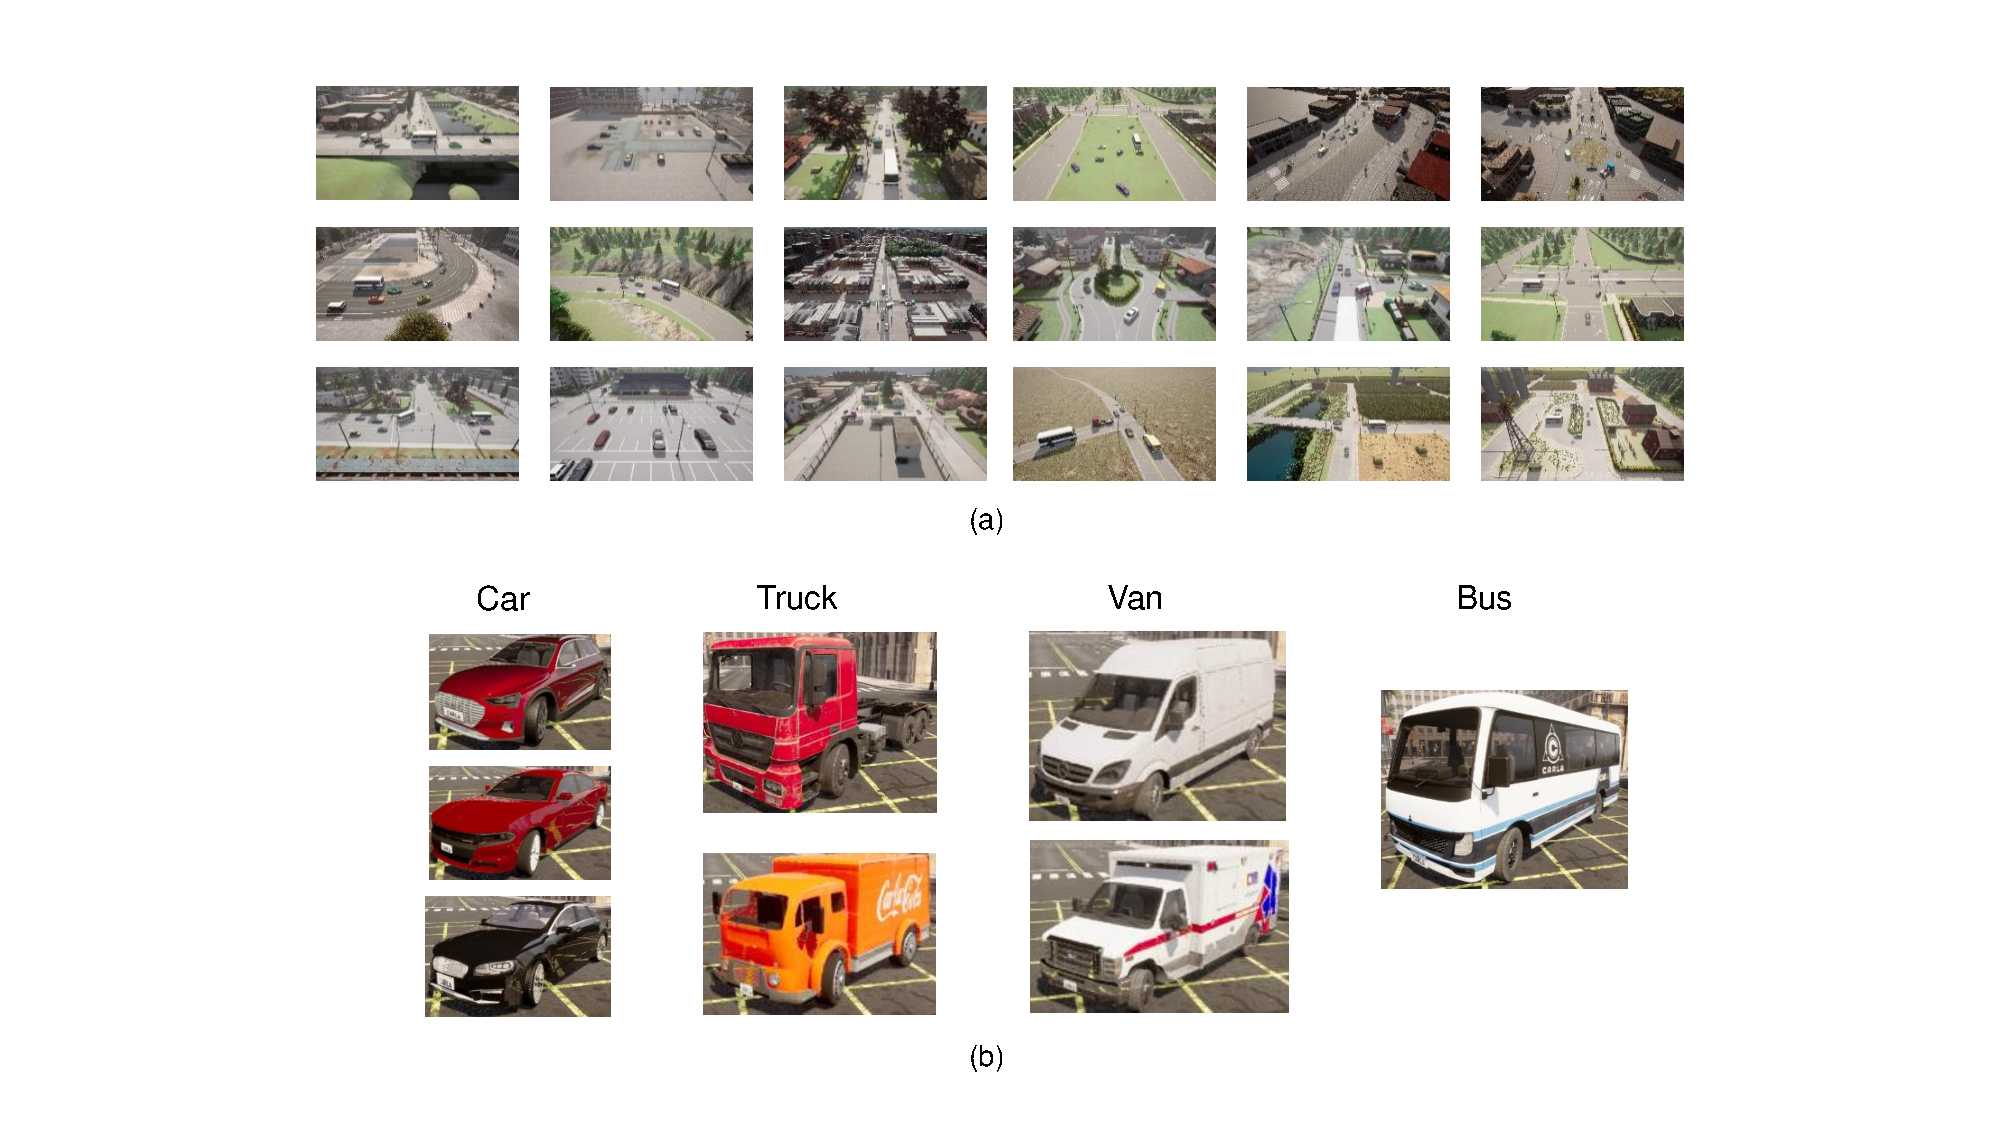
\includegraphics[width=0.45\textwidth]{fig/dataset.pdf}
    \caption{The CARLA-AOD Dataset. (a) Sample of Scenarios of the CARLA-AOD. (b) Categories of the CARLA-AOD Dataset.}
    \label{dataset}
\end{figure}

\begin{figure}[!t]
    \centering
    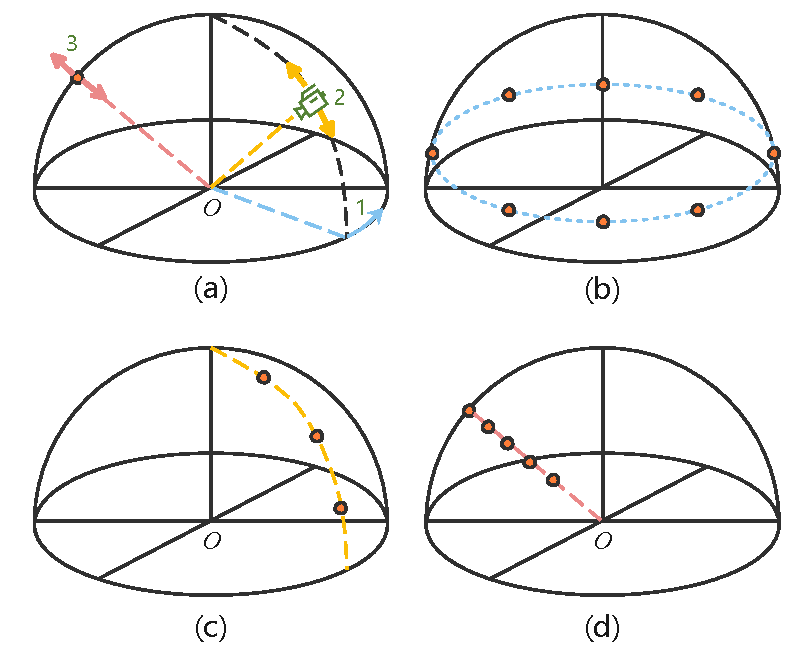
\includegraphics[width=0.45\textwidth]{fig/Acquisition.pdf}
    \caption{The CARLA-AOD Data Acquisition Mode. (a) Overall Data Collection Scheme. (b) Longitude-based Sampling Strategy. (c) Latitude-based Sampling Strategy. (d) Scale-based Sampling Strategy.}
    \label{Acquisition}
\end{figure}

In each scenario, vehicles are randomly placed at multiple locations, with vehicle types randomly selected from four categories: cars, trucks, vans, and buses. Different colors are randomly assigned to each vehicle to simulate real-world diversity. The vehicles are positioned with appropriate orientations to maintain realistic traffic distribution while ensuring they can be observed from multiple angles by the sensors.

To capture image data from various viewpoints and scales, we systematically adjust azimuth (longitude), elevation (latitude), and distance (scale) of the sensor relative to the camera center, as shown in Fig. \ref{Acquisition}. The azimuth settings cover a complete 360-degree range at 45-degree intervals, resulting in 8 different longitude angles. The elevation angles are set at three levels: 30, 45, and 60 degrees, covering different vertical perspectives. At each sensor position, five different distances (40m, 50m, 60m, 70m, and 80m) are used to generate various scaling effects. This configuration enables us to collect 120 images per scenario, combining 24 different viewpoint combinations with 5 scales.

During the collection process, the sensors not only record images but also generate corresponding vehicle labels for each image, including vehicle categories and bounding boxes. This information serves as the foundation for subsequent object detection tasks. The collection process maintains consistent operational procedures across all scenarios to ensure high data consistency and comparability, thereby enhancing applicability of the dataset across different models and algorithms.

The proposed CARLA-AOD dataset offers significant advantages over existing SA and VP datasets for AOD research. As shown in Table \ref{Datasets Compare}, CARLA-AOD provides greater scenario diversity, encompassing urban, town, and country environments, compared to SA and VP's limited airport and park scenarios respectively. Additionally, CARLA-AOD features 33 instances across 4 categories, substantially more than SA (12 instances, 12 categories) and VP (5 instances, 5 categories), enabling more robust model training and evaluation. Furthermore, while SA and VP are limited to upper quarter hemisphere coverage, CARLA-AOD offers full hemisphere coverage, providing a more comprehensive representation of the surveillance environment. These enhancements ensure thorough testing of active detection algorithms under diverse real-world conditions.

The CARLA-AOD dataset presents a more challenging and realistic benchmark for AOD research, with its diverse scenarios, increased object instances, and full hemisphere coverage, making it a valuable and impactful addition to the existing datasets in this domain. 

\begin{table*}[!t]
\renewcommand{\arraystretch}{1.5}
\caption{Comparison of Active Object Detection Datasets.}
\label{Datasets Compare}
\centering
\scalebox{0.95}{
\begin{tabular}{ccccccccc}

\toprule[1.5pt]
Datasets & Image Count & Categories & Instance & Views & Scales & Brightness & Coverage Area & Scenario Diversity \\ \hline
SA & 4500 & 12 & 12 & 10 & 5 & / & Quarter Hemisphere & Airport scenarios \\
VP & 5000 & 5 & 5 & 10 & 5 & 5 & Quarter Hemisphere & Parks scenarios \\
CARLA-AOD & 2160 & 4 & 33 & 24 & 5 & / & Full Hemisphere & Urban, Town and Country scenarios \\
\midrule[1.5pt]
\end{tabular}
}
\end{table*}

\begin{table*}[!]
  \centering
  \caption{mAP Performance of Various AOD Algorithms with Different Object Detectors on SA, VP and CARLA-AOD Datasets.}
    \label{compare}%
    \scalebox{0.85}{
    \begin{tabular}{c|cccc|cccc|cccc}
    \toprule[1.5pt]
          & \multicolumn{4}{c|}{SA}        & \multicolumn{4}{c|}{VP}       & \multicolumn{4}{c}{CARLA-AOD} \\ \hline
    Detectors & Original & DCCL  & Behavior Clone & Ours  & Original & DCCL  & Behavior Clone & Ours  & Original & DCCL  & Behavior Clone & Ours \\ \hline
    FCOS \cite{fcos2022b}  & 0.676  & 0.733  & 0.805  & \textbf{ 0.827 } & 0.669  & 0.797  & 0.800  & \textbf{0.831}  & 0.808  & 0.831  & 0.857  & \textbf{ 0.873 } \\
    ATSS \cite{bridging2020}  & 0.699  & 0.765  & 0.798  & \textbf{ 0.825 }  & 0.729  & \textbf{0.871}  & 0.808 & 0.833  & 0.809  & 0.839  & \textbf{ 0.847 } & 0.845 \\ 
    YOLOX \cite{yolox2021} & 0.668  & 0.781  & 0.774  & \textbf{ 0.793 } & 0.677  & 0.850  & 0.794  & \textbf{0.854}  & 0.632  & 0.709  & 0.680  & \textbf{ 0.711 } \\
    RTMDet \cite{rtmdet2022} & 0.699  & 0.765  & 0.798  & \textbf{ 0.825 } & 0.661  & \textbf{0.838}  & 0.811  & 0.831  & 0.717  & 0.758  & 0.761  & \textbf{ 0.777 } \\
    CenterNet \cite{objects2019} & 0.719  & \textbf{0.806}  & 0.783  & 0.799  & 0.768  & 0.857  & 0.868  & \textbf{0.880}  &  0.752  & \textbf{ 0.821 } & 0.783  & 0.805 \\ 
    RetinaNet \cite{focal2017} & 0.681  & 0.833  & 0.829  & \textbf{ 0.841 }  & 0.622  & 0.771  & 0.770  & \textbf{0.791}  &  0.765  & 0.795  & 0.771  & \textbf{ 0.844 } \\ 
    LibraRCNN \cite{libra2019} & 0.717  & 0.749  & 0.837  & \textbf{ 0.844 }  & 0.680  & 0.758  & 0.765  & \textbf{0.799}  &  0.743  & 0.779  & \textbf{ 0.785 } & 0.780 \\ 
    FasterRCNN \cite{faster2015a} & 0.716  & 0.756  & 0.834  & \textbf{ 0.836 }  & 0.687  & \textbf{0.811}  & 0.777  & 0.796  & 0.806  & \textbf{0.835}  & 0.821  & 0.828 \\ 
    \midrule[1.5pt]
    \end{tabular}%
    }

\end{table*}%







\subsection{Experimental Details}
\subsubsection{Dataset and Preprocessing}
In our experiments, we evaluate the performance of the proposed CARLA-AOD dataset in comparison to the existing SA and VP datasets. For the SA dataset and VP datasets, we use their original data splits, while for CARLA-AOD, we use a 3:2 ratio to divide the training and test sets.

To ensure compatibility with existing object detection frameworks, we utilized the MMDetection \cite{mmdetection} framework for detector pretraining and adopted its default preprocessing and data augmentation settings, which vary depending on the specific detector. For the FCOS detector \cite{fcos2022b} used in our primary experiments, this included resizing images to maintain an aspect ratio with the shorter side at 800 pixels and the longer side not exceeding 1333 pixels, random flipping with a probability of 0.5, photometric distortion, and normalization using ImageNet mean and standard deviation values. We maintained this default configuration across all detectors to ensure fair comparison and demonstrate our method's adaptability to different detection architectures.

\subsubsection{Implementation Environment}
All experiments were conducted using Python 3.8.17 and CUDA 11.3 on a workstation equipped with an Intel Xeon E5-2620 processor and 128GB of RAM. During the training phase, we use an NVIDIA GeForce RTX Titan GPU. 

\subsubsection{Computational Considerations}
It is important to note that the training time and memory requirements can vary significantly depending on the choice of object detection model and the dataset being used. This is due to the dependence of the model on the detector features as input, as well as differences in the sample size and difficulty of the datasets. For the FCOS detector on the CARLA-AOD dataset, the training process consists of two stages: imitation learning and reinforcement learning fine-tuning. The imitation learning stage takes approximately 6 hours, while the reinforcement learning fine-tuning requires an additional 5 hours.   

Beyond training time, memory consumption represents another significant consideration in our approach.  The feature-based nature of our model creates substantial memory demands, as it necessitates storing the detector features for each image in memory to enable efficient feature retrieval during training.  As a consequence, this approach results in a relatively high memory footprint of around 30 GB.
To mitigate the memory usage, an alternative approach involves computing the detector features on-the-fly during training, rather than storing them in memory.  This trade-off between training time and memory consumption should be considered when deploying the models in resource-constrained environments.

\subsubsection{Optimization Parameters}
In this study, we used Adam as the optimizer with a learning rate of 0.001 and weight decay of 0.01. We maintained a consistent batch size of 16 across all experiments. For the reinforcement learning component, we employed a discount factor $\gamma$ of 0.98, and initialized the exploration probability $\epsilon$ at 0.1, which gradually decreased to 0.01 during the training process. The maximum number of training steps was configured to 150,000. The optimal values for learning rate $lr$ and discount factor $\gamma$ were determined through grid search experiments, which are detailed in Section \ref{Hyperparameter Settings}.

\subsubsection{Evaluation Methodology}
In terms of evaluation metrics, we use mAP to assess model performance and the number of frames inferred per second (FPS) as the speed indicator.  Our evaluation process involves starting from any image in the dataset and iteratively selecting the next camera state until the model outputs a 'stop' action or the number of steps exceeds 10. At each time step, based on selection results of the model, we generate a new combination of images equal in size to the original dataset, where each image represents the newest state reached from different starting points. The object detector then performs detection on each image in this new combination, and the overall mAP is calculated to evaluate performance of the model.  The number of steps that the model processes per second serves as our speed indicator.



\begin{figure*}[!t]
    \centering
    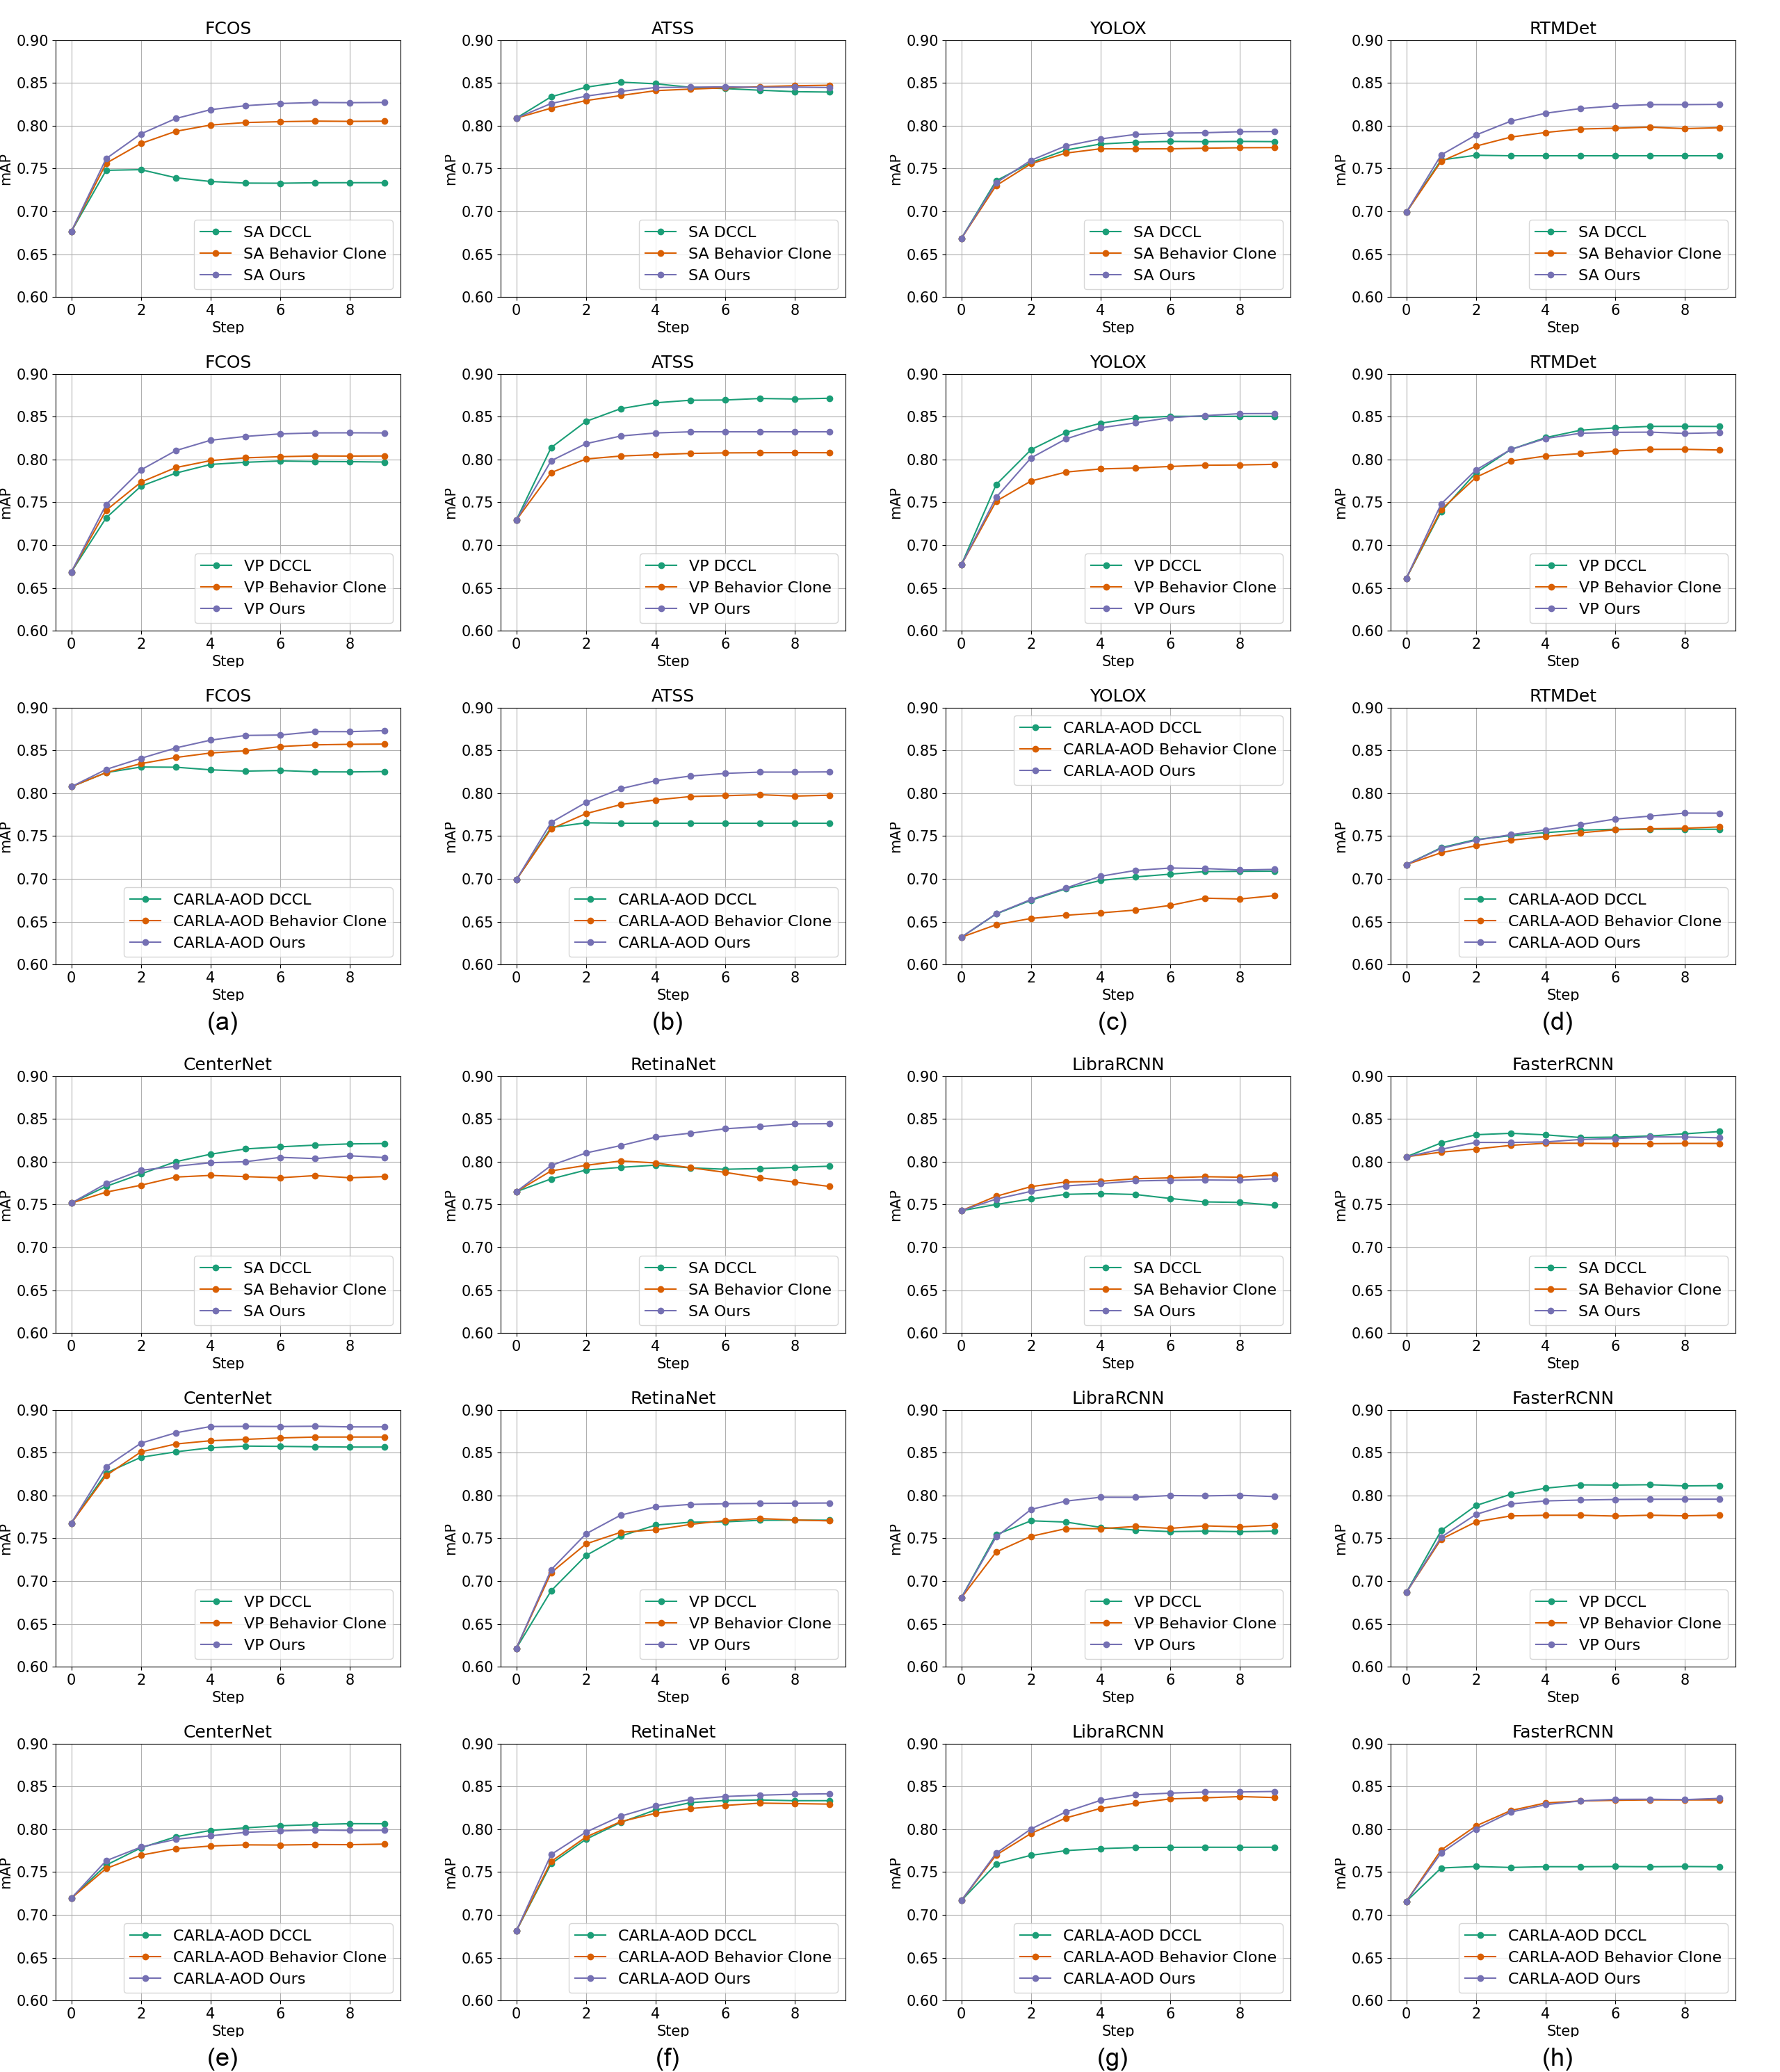
\includegraphics[width=1.0\textwidth]{fig/mAPs.png}
    \caption{mAP Curves of Detectors on Datasets. (a) mAP Curves on FCOS. (b) mAP Curves on ATSS. (c) mAP Curves on YOLOX. (d) mAP Curves on RTMDet. (e) mAP Curves on CenterNet. (f) mAP Curves on RetinaNet. (g) mAP Curves on LibraRCNN. (h) mAP Curves on FasterRCNN.}
    \label{mAPs}
\end{figure*}

\begin{figure*}[!t]
    \centering
    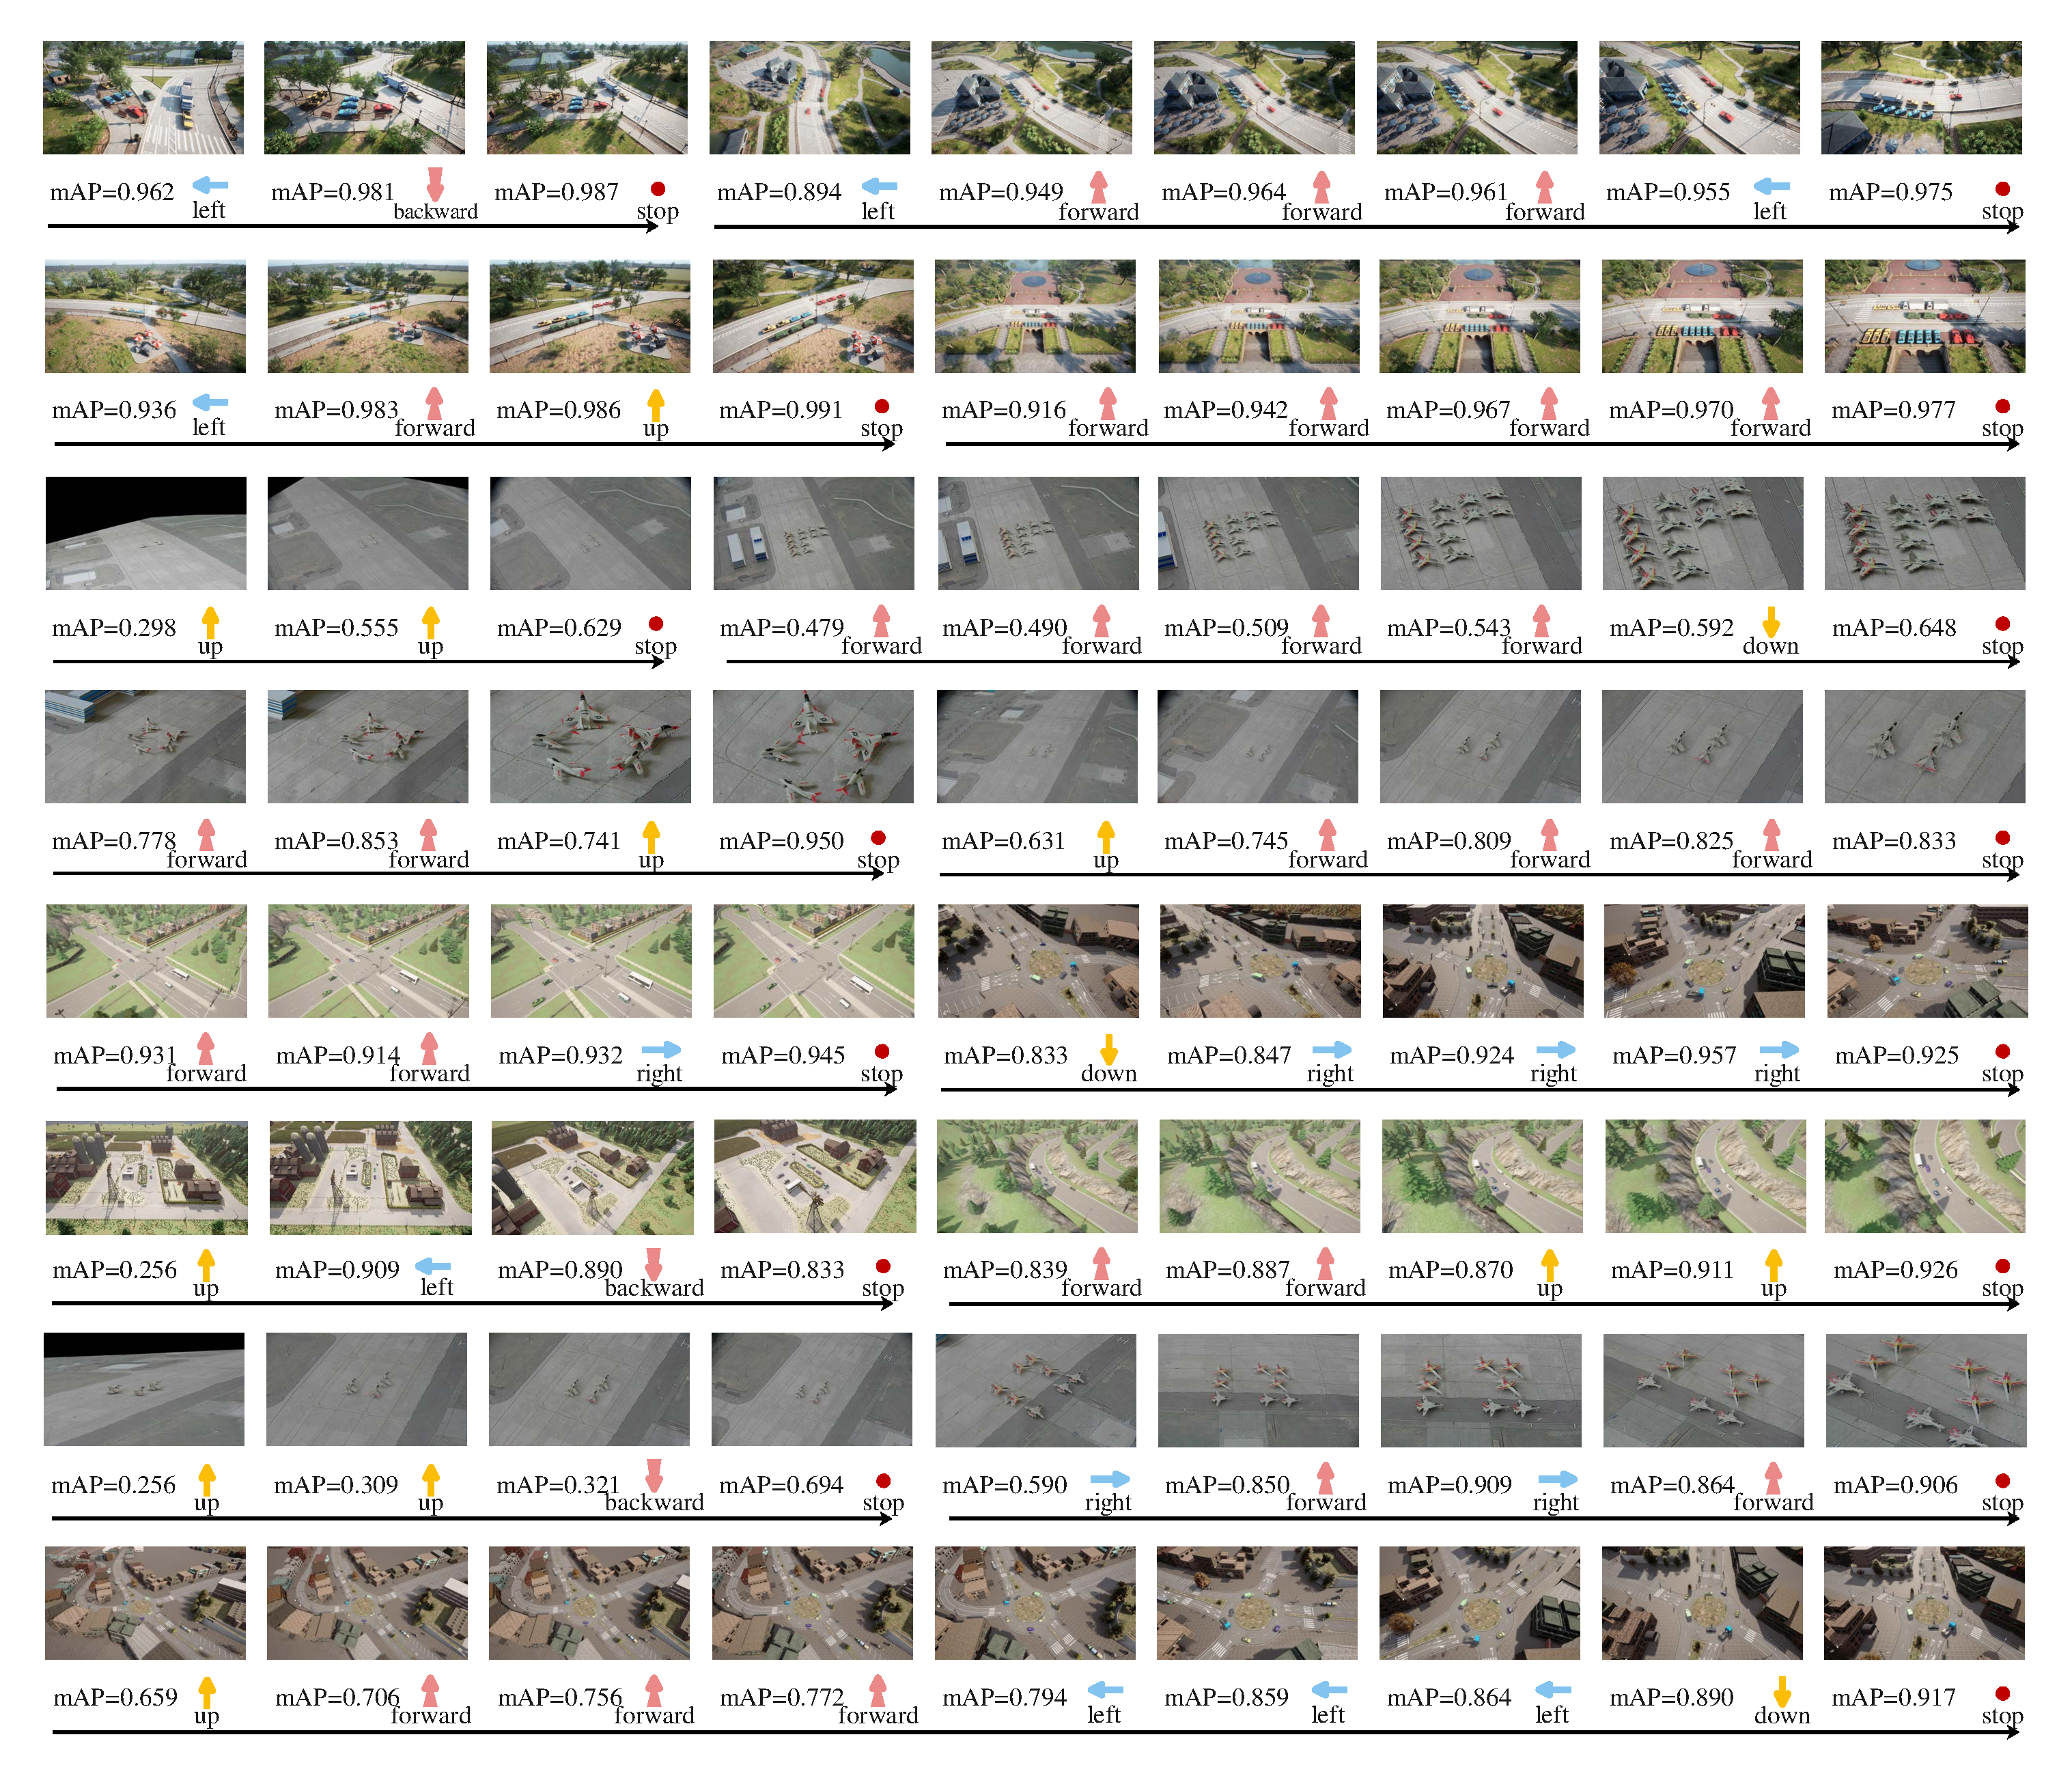
\includegraphics[clip=true, width=1.0\textwidth]{fig/visualization.pdf}
    \caption{Results of the Proposed Method in SA, VP and CARLA-AOD with Action Sequence.}
    \label{visualization}
\end{figure*}

\subsection{Result and Analysis}
\subsubsection{Performance in Different Datasets and Detectors}
Table \ref{compare} presents the evaluation results of our proposed model on three datasets, comparing its performance after behavior cloning and final training with the DCCL algorithm. We employ eight object detectors as our base models: FCOS, ATSS \cite{bridging2020}, YOLOX \cite{yolox2021}, RTMDet \cite{rtmdet2022}, CenterNet \cite{objects2019}, RetinaNet \cite{focal2017}, LibraRCNN \cite{libra2019}, FasterRCNN \cite{faster2015a}. The \textit{Original} column represents the initial performance of these detectors without any AOD enhancements.
The experimental results show that our proposed active target detection algorithm has achieved significant performance improvements on multiple datasets and target detectors.

In the SA dataset, our method demonstrated significant improvements for most detectors. FCOS and RetinaNet showed notable gains of 15.1\% and 16.0\% respectively, while LibraRCNN and FasterRCNN improved by 12.7\% and 12.0\%. Even for detectors with already competitive baseline performance, our method achieved consistent improvements.

In the VP dataset, the results demonstrate substantial performance enhancements across different architectures. YOLOX and RTMDet showed remarkable gains of 17.7\% and 17.0\% respectively, while CenterNet exhibited an 11.2\% increase in mAP. The ATSS detector, with its relatively higher baseline performance, still showed significant enhancement with a 14.2\% improvement from 0.729 to 0.871 mAP.

In the CARLA-AOD dataset, we observed consistent performance improvements across detector types. RetinaNet improved by 7.9\% and FCOS by 6.5\%, while CenterNet and LibraRCNN gained 5.3\% and 3.7\% respectively. For ATSS, which had a high baseline performance of 0.809, our approach still improved performance to 0.847 with behavior cloning, demonstrating good adaptability across different scenarios.


The variations in performance across datasets reveal patterns related to their fundamental complexity differences. In the SA dataset's structured airport environment, FCOS shows a remarkable improvement from 0.676 to 0.827 mAP, while LibraRCNN and RetinaNet advance from 0.717 to 0.844 mAP and 0.681 to 0.841 mAP respectively. These specific gains demonstrate our method's effectiveness on both anchor-free and anchor-based architectures in controlled settings.
The VP dataset analysis reveals distinct patterns in environments with moderate complexity. YOLOX improves significantly from 0.677 to 0.854 mAP, and CenterNet from 0.768 to 0.880 mAP. While DCCL achieves 0.871 mAP with ATSS, outperforming our final result of 0.833 mAP, our method delivers more consistent improvements across most other architectures, particularly with FCOS and RetinaNet reaching 0.831 mAP and 0.791 mAP respectively.

In the complex CARLA-AOD dataset with diverse scenarios, FCOS improves from 0.808 to 0.873 mAP and RetinaNet from 0.765 to 0.844 mAP. Notably, for CenterNet (0.752 to 0.805 mAP) and LibraRCNN (0.743 to 0.780 mAP), the behavior cloning phase already yields strong results of 0.783 mAP and 0.785 mAP respectively. Compared to DCCL, our method shows superior performance on most detectors, though DCCL occasionally performs better, such as with FasterRCNN (0.835 mAP versus our 0.828 mAP).

These nuanced performance patterns across datasets validate our approach's adaptive utility in varying environmental complexities. Our final method consistently outperforms both the original detectors and the behavior cloning intermediary stage in most scenarios, confirming the effectiveness of our complete pipeline. The comparative analysis with DCCL further highlights the strengths of our approach, particularly in maintaining strong performance across diverse detection architectures and environmental challenges. The robust improvements across almost all detector-dataset combinations underscore our method's versatility and practical value in real-world applications where varying levels of environmental complexity are encountered.
\begin{table}[!t]
    \caption{FPS of Various AOD Algorithms with Different Object Detectors.}
    \label{Fps}
    \centering
    \begin{tabular}{>{\centering\arraybackslash}m{2.5cm} >{\centering\arraybackslash}m{1.75cm} >{\centering\arraybackslash}m{1.75cm}}
    \toprule[1.5pt]
    Detector & DCCL  & Ours \\ \hline
    FCOS \cite{fcos2022b}  & 12.7  & \textbf{19.8}  \\
    ATSS \cite{bridging2020} &  13.2  & \textbf{18.3}  \\
    YOLOX \cite{yolox2021} & 14.7  & \textbf{21.2}  \\
    RtmDet \cite{rtmdet2022} & 12.2  & \textbf{20.1} \\
    CenterNet \cite{objects2019} & 12.7  & \textbf{20.4} \\
    RetinaNet \cite{focal2017} & 10.8  & \textbf{20.4} \\
    LibraRCNN \cite{libra2019} & 11.0  & \textbf{17.2} \\
    FasterRCNN \cite{faster2015a} & 13.1  & \textbf{22.6} \\
    \midrule[1.5pt]
    \end{tabular}%
\end{table}

\begin{figure*}[!t]
    \centering
    \includegraphics[clip=true, width=1.0\textwidth]{fig/complex.pdf}
    \caption{Performance of the Proposed Method in Complex Scenarios.}
    \label{complex}
\end{figure*}

\begin{figure*}[!t]
    \centering
    \includegraphics[clip=true, width=1.0\textwidth]{fig/failure.pdf}
    \caption{Visualization results of failure cases}
    \label{failure}
\end{figure*}


From the mAP curve in Fig. \ref{mAPs}, most detectors improved rapidly in the first 2-4 steps and then leveled off. Our method usually converges to higher mAP values than other methods, demonstrating the effectiveness of our proposed reinforcement learning fine-tuning strategy.
Behavior cloning , as an intermediate process, significantly improved detection performance in most cases. The subsequent reinforcement learning fine-tuning phase further optimizes the results, confirming the necessity of our complete algorithm flow. For example, in the CARLA-AOD dataset, RetinaNet achieved an additional 7.3\% improvement from behavior cloning to the final result stage.  

Beyond accuracy improvements, our method also demonstrates significant gains in computational efficiency. Table \ref{Fps} shows that our algorithm achieves a substantial increase in inference speed compared to DCCL, with an average 60.2\% improvement in steps per second across all eight detectors.



\subsubsection{Visualization Result in Different Datasets}
Visualization results and the decision process are shown in Fig. \ref{visualization}, illustrating the active target detection process with a sequence of images and corresponding actions. Our algorithm demonstrates significant and consistent mAP improvements, validating the effectiveness of the proposed method.

As shown in Fig. \ref{complex}, in the case where the target is initially occluded or surrounded by complex background clutter, the UAV adjusts its camera angle and position, indicated by actions such as up, left, to navigate around the occluding obstacles and reach a more advantageous viewpoint. The model further optimizes detection by adjusting scale through forward or backward movements, fine-tuning the camera perspective until the target becomes clearly visible. The effectiveness of this approach is validated by the high mAP scores recorded during these intermediate steps.
The final stop action is only triggered once the model is confident it has successfully detected the target. This demonstrates capability of the model to dynamically adapt its sensing strategy to handle challenging environmental conditions.

Regarding occlusion situations, the first to third rows in Fig. \ref{complex} represent three scenarios with initial occlusion rates ranging from high to low. For medium and low occlusion rates, the model tends to prefer action up to increase latitude $\theta$. This approach can effectively address occlusions caused by obstacles and avoids potential new occlusions that might result from adjusting the azimuth angle by action left or right. However, for high occlusion rates, while increasing latitude $\theta$ can somewhat reduce the occlusion of targets by obstacles, its effectiveness is often limited. In such cases, the model tends to choose left or right to attempt to navigate around the obstacles.

In the model inference process, a small number of failure cases were observed. Fig. \ref{failure} illustrates two representative failure scenarios. The first row demonstrates instances where detector performance declined after reaching a relative peak. This phenomenon primarily occurs because the model tends to resort to commonly used forward actions to adjust camera configuration when encountering unfamiliar scenes, indicating room for improvement in the model's generalization capabilities. The second row depicts situations where the model became trapped in local optima, with dashed lines representing potential action adjustments that could escape these suboptimal states. These scenarios suggest that data augmentation techniques and adaptive reward functions may be necessary to further enhance model robustness.

While these failure cases reveal certain limitations, they also provide clear directions for future improvements. Through data augmentation techniques and adaptive reward functions, we are confident that model robustness and generalization capabilities can be further enhanced. These results collectively demonstrate that our proposed model achieves state-of-the-art accuracy in AOD tasks while delivering substantial computational efficiency improvements. 
This combination of high accuracy and fast inference speed makes our method ideal for real-time applications in UAV-based object detection scenarios.


\begin{table}[!]
  \centering
  \caption{mAP Performance of Ablation Experiment on Discount Factor and Learning Rate.}
    {\begin{tabular}{ccc}
    \toprule[1.5pt]
    \multicolumn{1}{l}{Discount Factor} & \multicolumn{1}{l}{Learning Rate} & \multicolumn{1}{l}{Performance} \\ \hline
    \multirow{5}[0]{*}{0.97} & 0.01  & 0.841 \\
          & 0.005 & 0.842 \\
          & 0.001 & 0.846 \\
          & 0.0005 & 0.821 \\
          & 0.0001 & 0.837 \\ \hline
    \multirow{5}[0]{*}{0.98} & 0.01  & 0.856 \\
          & 0.005 & 0.849 \\
          & 0.001 & 0.873 \\
          & 0.0005 & 0.845 \\
          & 0.0001 & 0.841 \\ \hline
    \multirow{5}[0]{*}{0.99} & 0.01  & 0.863 \\
          & 0.005 & 0.862 \\
          & 0.001 & 0.845 \\
          & 0.0005 & 0.847 \\
          & 0.0001 & 0.847 \\ 
    \midrule[1.5pt]
    \end{tabular}%
}
  \label{hyperparameter}%
\end{table}%





\subsection{Ablation Study}

To thoroughly evaluate our proposed method, we conducted comprehensive ablation studies focusing on three aspects: (1) hyperparameter settings, including the discount factor and learning rate; (2) the impact of different numbers of feature layers on detection performance and computational efficiency; and (3) the effectiveness of key components in our framework, including shallow features, action prediction module, and behavior cloning.

\subsubsection{Hyperparameter Settings}
\label{Hyperparameter Settings}
We conducted a comprehensive sensitivity analysis to investigate the optimal hyperparameter configuration through a grid search. As shown in Table \ref{hyperparameter}, we explored three values for the discount factor ($\gamma$ of 0.97, 0.98, and 0.99) and five learning rates ($lr$ values of 0.01, 0.005, 0.001, 0.0005, and 0.0001). This thorough evaluation helps us better assess the robustness of our model under varied parameter settings.

The results demonstrate that a combination with $\gamma$ of 0.98 and learning rate of 0.001 achieved the best performance with a score of 0.873. For the discount factor, we observe that higher values with $\gamma$ of 0.99 generally outperform both moderate values with $\gamma$ of 0.98 and lower values with $\gamma$ of 0.97 across most learning rates, except for the optimal combination with $lr$ of 0.001 and $\gamma$ of 0.98. This indicates our model typically benefits from prioritizing future rewards, though the optimal configuration depends on the specific learning rate.

The performance exhibits a clear pattern with respect to learning rate, with an $lr$ of 0.001 being optimal for a $\gamma$ value of 0.98, while higher learning rates with $lr$ of 0.01 work better for a $\gamma$ of 0.99. This suggests an interaction effect between these parameters, where models with higher discount factors benefit from more aggressive learning steps. The model shows particular sensitivity to very small learning rates, with an $lr$ of 0.0005 producing the worst performance of 0.821 when combined with a $\gamma$ of 0.97.

Our sensitivity analysis confirms the robustness of this approach. Performance remains relatively stable above 0.84 in most configurations across a wide range of hyperparameter values, with only specific combinations showing significant degradation. The optimal configuration with $\gamma$ of 0.98 and learning rate of 0.001 provides the right balance between learning speed and stability, validating the final choice for model deployment.

\subsubsection{Different Numbers of Feature Layers}
We analyzed the impact of utilizing different numbers of feature layers from the FPN detector on both model performance and computational efficiency across three datasets, as shown in Table \ref{layers ablation}. The experimental results demonstrate that for simpler scenarios represented in the SA and VP datasets, utilizing a single high-resolution feature layer achieves competitive performance while maintaining optimal computational efficiency.   Specifically, on the SA dataset, our approach with a single feature layer achieves an impressive performance of 0.832, which is significantly higher than the original baseline of 0.676. Similarly, for the VP dataset, the single-layer configuration yields a strong performance of 0.824, substantially outperforming the original baseline of 0.669.

When considering more complex environments as represented in the CARLA-AOD dataset, incorporating additional feature layers shows potential benefits.   The performance improves from 0.830 with a single layer to 0.851 with two layers, suggesting that the integration of multi-scale features can better capture the diverse object instances and complex scenario compositions present in this dataset.   However, it is worth noting that increasing the number of feature layers beyond two yields diminishing returns in performance while significantly impacting the computational efficiency, as evidenced by the dramatic decrease in FPS from 19.8 with a single layer to 12.7 with five layers.

\begin{table}[!]
  \centering
  \caption{mAP Performance of Ablation Experiment on the Number of Feature Layers.}
    \scalebox{0.9}{\begin{tabular}{c|c|c|c|c|c|c|c}
    \toprule[1.5pt]
          & \multicolumn{2}{c|}{SA} & \multicolumn{2}{c|}{VP} & \multicolumn{2}{c|}{CARLA-AOD} &  \\ \hline
    Layers & Original & Ours  & Original & Ours  & Original & Ours  & FPS \\ \hline
    1     & \multirow{5}[0]{*}{0.676} & 0.832  & \multirow{5}[0]{*}{0.669} & 0.824  & \multirow{5}[0]{*}{0.808} & 0.830    & 19.8 \\
    2     &       & 0.829  &       & 0.834  &       & 0.851  & 17.5 \\
    3     &       & 0.827  &       & 0.794  &       & 0.846  & 14.4 \\
    4     &       & 0.832  &       & 0.812  &       & 0.844  & 12.9 \\
    5     &       & 0.829  &       & 0.801  &       & 0.849  & 12.7 \\
    \midrule[1.5pt]
    \end{tabular}%
}
  \label{layers ablation}%
\end{table}%



The empirical findings support our design choice of utilizing a single high-resolution feature layer in our final model architecture.   This decision represents an optimal trade-off between model performance and computational efficiency, particularly crucial for real-world AOD applications where real-time processing capabilities are essential.   For simpler scenarios, this configuration achieves state-of-the-art performance while maintaining high FPS, and even for complex environments, the performance degradation is relatively small compared to multi-layer alternatives while offering substantially better computational efficiency.

\subsubsection{Contributions of Each Component}
Beyond the number of feature layers, we further investigated the individual contributions of each component in our proposed approach to assess their impact on AOD performance, as shown in Table \ref{ablation}. The experimental results demonstrate that each module significantly improves the performance of AOD. After incorporating shallow features, the performance on the SA dataset increased from 67.6\% to 81.3\%, an improvement of 13.7 percentage points; on the CARLA-AOD dataset, performance improved from 80.8\% to 82.8\%, an increase of 2 percentage points. This indicates that shallow features play a crucial role in enhancing object detection performance, especially in the SA dataset.

\begin{table}[!]
  \centering
  \caption{mAP Performance of Ablation Experiment on Components of Models.}
  \scalebox{0.85}{
    \begin{tabular}{cccc|ccc}
    \toprule[1.5pt]
    \multicolumn{4}{c|}{Method} & \multicolumn{3}{c}{Datasets}\\ \hline
    Original & \makecell{Shallow \\ Feature} & \makecell{Action \\ Prediction} & \makecell{Behavior \\ Clone} & SA  & VP   & CARLA-AOD \\ \hline
    \checkmark     &       &       &       & 0.676  &0.669 & 0.808 \\
    \checkmark     & \checkmark      &       &       & 0.813 &0.824 & 0.828 \\
    \checkmark     & \checkmark      & \checkmark      &       & 0.826 &0.827 & 0.835 \\
    \checkmark     & \checkmark      & \checkmark      & \checkmark      & 0.827 &0.831 & 0.873 \\
    \midrule[1.5pt]
    \end{tabular}%
}
  \label{ablation}%
\end{table}%

Building upon the shallow features, the addition of the action prediction module further improved performance on both datasets. On the SA dataset, performance increased to 82.6\%, a 1.3 percentage point improvement compared to using shallow features alone; on the CARLA-AOD dataset, performance rose to 83.5\%, a 0.7 percentage point increase. This suggests that the action prediction module can enhance feature extraction capabilities of the model, thereby further improving performance. Besides, action prediction task enhances robustness against dynamic background variations by implicitly learning viewpoint transition patterns.

Finally, the incorporation of behavior cloning demonstrates particularly significant value in complex operational environments. While the SA dataset shows modest improvement (82.6\% to 82.7\%), CARLA-AOD achieves a substantial 3.8 percentage point gain (83.5\% to 87.3\%), directly validating the component's effectiveness in cluttered scenarios. This performance leap stems from the dual mechanism of behavior cloning: the A-star-generated expert trajectories provide stable initialization that mitigates "sparse reward" caused by random exploration in complex background environments, and subsequent reinforcement learning fine-tuning enables learning general strategies. This experimental evidence confirms that behavior cloning facilitates generalized strategy learning through expert imitation while maintaining adaptability to complex UAV scenarios.

Although shallow features brought significant improvements on the SA and VP datasets (13.7 and 15.5 percentage points, respectively), the improvement on the CARLA-AOD dataset was relatively modest (2 percentage points).   This disparity likely stems from the fundamental differences between the three datasets.   The SA and VP datasets contain fewer target instances with relatively simple backgrounds, characteristics that can be well captured in shallow network layers.   In contrast, the CARLA-AOD dataset encompasses more diverse target instances and more complex urban, town, and rural environments, potentially requiring deeper features for effective target discrimination.

As previously noted, behavior cloning yielded substantial improvements on the CARLA-AOD dataset (3.8 percentage points) while showing minimal gains on the SA and VP datasets (0.1 and 0.4 percentage points, respectively).   This may be attributed to the CARLA-AOD dataset containing more complex and diverse scenarios that require more sophisticated decision-making strategies.   Behavior cloning allows the model to learn these complex strategies from expert demonstrations, hence performing better on this dataset.   In comparison, the scenarios in SA and VP datasets may be relatively straightforward, making direct reinforcement learning strategies sufficiently effective and limiting the additional benefits from behavior cloning.

While our method demonstrated performance improvements across all three datasets, the contributions of different components indeed varied across datasets.   This suggests that certain aspects of the algorithm may need to be tailored for specific types of scenarios to achieve optimal performance.   Future work could explore ways to enhance the generalizability of the algorithm, such as introducing a more adaptive feature layer selection mechanism or designing behavior cloning strategies that better generalize across different scenarios.

\section{Conclusion}
This paper proposes an improved approach to AOD in UAV remote sensing imagery, addressing the fundamental challenges in UAV-based object detection that were identified in our introduction.  Our method effectively tackles the primary limitations of passive processing approaches, particularly the challenges of multi-scale targets and partial occlusions that arise from varying UAV flight conditions.  Through a refined model architecture incorporating FPN features, an enhanced two-stage learning strategy combining expert policy generation with behavior cloning, and the comprehensive CARLA-AOD dataset, we demonstrate significant advances in AOD capabilities.

Experimental results show a 10.7\% improvement over the original detectors, and a 2.3\% improvement compared to the DCCL method. Moreover, the 60.2\% improvement in processing speed achieved by our method is particularly impactful, as it directly addresses a key challenge in UAV applications: the need for real-time or near-real-time object detection.

The enhanced inference speed of our method has profound practical implications, particularly in time-sensitive scenarios such as disaster response and surveillance operations. Rapid object detection is crucial for quickly assessing situations, locating targets, and coordinating efforts. In disaster response, near-real-time frame processing allows UAVs to swiftly identify affected areas, locate stranded individuals, and assess damage extent. This capability enables emergency responders to prioritize rescue efforts and allocate resources effectively. In surveillance operations, our method enables UAVs to cover larger areas and provide up-to-date information, enhancing situational awareness and decision-making. The improved efficiency also translates to better utilization of limited UAV flight time and battery life, allowing for advanced capabilities without compromising mission duration or operational range. Overall, our method significantly enhances UAV operations in critical situations.

Looking beyond UAV applications, our innovations in combining FPN features with behavior cloning and reinforcement learning present promising opportunities for advancing AOD in other domains requiring adaptive perception strategies.  Future research could explore the application of our approach to different scenarios and further optimize the balance between detection accuracy and computational efficiency.

\section{Limitations}
Despite the promising results of our approach, several limitations warrant acknowledgment. First, our model occasionally exhibits algorithmic limitations when encountering complex scenes. As illustrated in Fig. \ref{failure}, performance degradation occurs after reaching peak performance in unfamiliar environments with multiple objects at varying scales or partial occlusions. The model tends to become trapped in local optima during decision-making and resort to commonly used forward actions, indicating that while our approach improves upon passive detection methods, it still faces challenges in highly complex scenarios.

Second, our current implementation faces significant domain adaptability challenges when transferred to real-world environments that differ from simulation. The model's performance heavily depends on the characteristics of the training environments, and the simulation-to-reality gap might require substantial retraining or fine-tuning. This generalization limitation suggests a need for more diverse and realistic training scenarios to better bridge the gap between simulation and actual deployment conditions.

Finally, real-world deployment faces practical constraints including computational resource limitations on UAV platforms, which may affect the real-time performance of our method despite the significant speed improvements we achieved. Energy consumption considerations and hardware compatibility issues also present challenges for practical implementation in resource-constrained UAV systems.

\section{Future Work}
While our current approach shows promising results for static object detection, several directions for future research warrant exploration. A primary challenge lies in the performance of the model on moving targets within dynamic environments. UAVs often operate in highly dynamic settings where objects of interest may shift or move unpredictably over time, presenting unique challenges for AOD which is typically designed for relatively stable targets. For example, in urban surveillance, vehicles and pedestrians move along various paths, making it difficult to maintain accurate detection and tracking. Additionally, environmental factors such as wind, rain, and varying lighting conditions can further complicate the detection process, leading to potential inaccuracies and missed detections. Moreover, practical deployment considerations such as computational resource constraints, and hardware limitations in real-world UAV systems need to be thoroughly addressed.

Our current study primarily focuses on AOD for multiple static objects of interest, leveraging the ability of the UAV to adjust camera angles and positions to improve detection accuracy. However, detecting multiple dynamic objects introduces significant challenges that warrant further investigation. These challenges include handling real-time adjustments to track various objects' movements along unique motion paths, managing UAV motion constraints, and addressing the unpredictable movement patterns of multiple targets. The complexity of these dynamic scenarios necessitates sophisticated control strategies that can balance detection accuracy with tracking capabilities while accounting for real-world system constraints such as battery life, processing power, and communication bandwidth.

For scenarios involving dynamic objects, we envision integrating active object tracking (AOT) techniques with our current AOD framework. While AOT traditionally focuses on single-object tracking through predictive modeling and real-time adjustments, we propose developing hybrid models that combine AOD and AOT capabilities. These hybrid systems would enable simultaneous handling of both static and dynamic objects within complex scenarios. Future research directions include developing adaptive algorithms for multi-object tracking under diverse motion patterns, optimizing UAV control strategies for combined tracking and detection performance, and investigating efficient resource allocation methods for real-time processing of dynamic scenes. Furthermore, we plan to explore robust deployment strategies that address practical challenges such as system resilience to environmental disturbances, optimization for edge computing platforms, and integration with existing UAV control systems.

A crucial direction for future work lies in validating our approach in real-world operational environments. We plan to conduct comprehensive field testing across diverse scenarios. These real-world evaluations will assess how our improvements in detection accuracy and computational efficiency translate to practical operational advantages. The validation process will involve collecting and analyzing real-world datasets, which may present unique challenges not encountered in controlled environments. This testing phase will be crucial for evaluating system robustness and reliability under actual deployment conditions, potentially leading to optimizations tailored to specific operational requirements. Furthermore, we will investigate the impact of environmental factors such as varying weather conditions, lighting changes, and complex urban landscapes on system performance.

Additionally, ethical considerations must be addressed for real-world deployment. Privacy protection requires implementing robust data anonymization techniques and establishing clear protocols for data collection and storage. The system should be enhanced with privacy-preserving features such as automatic masking of sensitive areas and strict access control mechanisms. Furthermore, responsible deployment guidelines need to be developed to prevent potential misuse while maintaining system effectiveness in legitimate applications. We also plan to develop comprehensive frameworks for assessing and mitigating potential societal impacts, ensuring transparent and accountable system operation while maintaining high performance standards.

The current study primarily focuses on UAV object detection scenarios at lower altitudes, where direct or lateral oblique viewing angles are common.  However, real-world UAV operations often involve cruising altitudes of 2000-3000 meters, resulting in predominantly top-down or high-angle oblique perspectives.  These high-altitude scenarios present unique challenges that warrant further investigation.  Future research should extend our approach to address these operational conditions through comprehensive dataset enhancement that incorporates more high-altitude aerial imagery with appropriate viewing angles typical of UAV cruise operations. These developments would significantly enhance the real-world applicability of our approach and better address the challenges faced in actual UAV deployment scenarios.

Future research could also explore applications in other domains and more advanced reinforcement learning algorithms, focusing on developing adaptive algorithms capable of handling both static and dynamic scenarios. These developments would contribute to more comprehensive and responsible UAV-based detection systems.



\bibliographystyle{IEEEtran}
\IEEEtriggeratref{99}
\bibliography{reference.bib}



\vfill

\end{document}


